% Options for packages loaded elsewhere
\PassOptionsToPackage{unicode}{hyperref}
\PassOptionsToPackage{hyphens}{url}
%
\documentclass[
]{article}
\usepackage{amsmath,amssymb}
\usepackage{lmodern}
\usepackage{iftex}
\ifPDFTeX
  \usepackage[T1]{fontenc}
  \usepackage[utf8]{inputenc}
  \usepackage{textcomp} % provide euro and other symbols
\else % if luatex or xetex
  \usepackage{unicode-math}
  \defaultfontfeatures{Scale=MatchLowercase}
  \defaultfontfeatures[\rmfamily]{Ligatures=TeX,Scale=1}
\fi
% Use upquote if available, for straight quotes in verbatim environments
\IfFileExists{upquote.sty}{\usepackage{upquote}}{}
\IfFileExists{microtype.sty}{% use microtype if available
  \usepackage[]{microtype}
  \UseMicrotypeSet[protrusion]{basicmath} % disable protrusion for tt fonts
}{}
\makeatletter
\@ifundefined{KOMAClassName}{% if non-KOMA class
  \IfFileExists{parskip.sty}{%
    \usepackage{parskip}
  }{% else
    \setlength{\parindent}{0pt}
    \setlength{\parskip}{6pt plus 2pt minus 1pt}}
}{% if KOMA class
  \KOMAoptions{parskip=half}}
\makeatother
\usepackage{xcolor}
\usepackage[margin=1in]{geometry}
\usepackage{color}
\usepackage{fancyvrb}
\newcommand{\VerbBar}{|}
\newcommand{\VERB}{\Verb[commandchars=\\\{\}]}
\DefineVerbatimEnvironment{Highlighting}{Verbatim}{commandchars=\\\{\}}
% Add ',fontsize=\small' for more characters per line
\usepackage{framed}
\definecolor{shadecolor}{RGB}{248,248,248}
\newenvironment{Shaded}{\begin{snugshade}}{\end{snugshade}}
\newcommand{\AlertTok}[1]{\textcolor[rgb]{0.94,0.16,0.16}{#1}}
\newcommand{\AnnotationTok}[1]{\textcolor[rgb]{0.56,0.35,0.01}{\textbf{\textit{#1}}}}
\newcommand{\AttributeTok}[1]{\textcolor[rgb]{0.77,0.63,0.00}{#1}}
\newcommand{\BaseNTok}[1]{\textcolor[rgb]{0.00,0.00,0.81}{#1}}
\newcommand{\BuiltInTok}[1]{#1}
\newcommand{\CharTok}[1]{\textcolor[rgb]{0.31,0.60,0.02}{#1}}
\newcommand{\CommentTok}[1]{\textcolor[rgb]{0.56,0.35,0.01}{\textit{#1}}}
\newcommand{\CommentVarTok}[1]{\textcolor[rgb]{0.56,0.35,0.01}{\textbf{\textit{#1}}}}
\newcommand{\ConstantTok}[1]{\textcolor[rgb]{0.00,0.00,0.00}{#1}}
\newcommand{\ControlFlowTok}[1]{\textcolor[rgb]{0.13,0.29,0.53}{\textbf{#1}}}
\newcommand{\DataTypeTok}[1]{\textcolor[rgb]{0.13,0.29,0.53}{#1}}
\newcommand{\DecValTok}[1]{\textcolor[rgb]{0.00,0.00,0.81}{#1}}
\newcommand{\DocumentationTok}[1]{\textcolor[rgb]{0.56,0.35,0.01}{\textbf{\textit{#1}}}}
\newcommand{\ErrorTok}[1]{\textcolor[rgb]{0.64,0.00,0.00}{\textbf{#1}}}
\newcommand{\ExtensionTok}[1]{#1}
\newcommand{\FloatTok}[1]{\textcolor[rgb]{0.00,0.00,0.81}{#1}}
\newcommand{\FunctionTok}[1]{\textcolor[rgb]{0.00,0.00,0.00}{#1}}
\newcommand{\ImportTok}[1]{#1}
\newcommand{\InformationTok}[1]{\textcolor[rgb]{0.56,0.35,0.01}{\textbf{\textit{#1}}}}
\newcommand{\KeywordTok}[1]{\textcolor[rgb]{0.13,0.29,0.53}{\textbf{#1}}}
\newcommand{\NormalTok}[1]{#1}
\newcommand{\OperatorTok}[1]{\textcolor[rgb]{0.81,0.36,0.00}{\textbf{#1}}}
\newcommand{\OtherTok}[1]{\textcolor[rgb]{0.56,0.35,0.01}{#1}}
\newcommand{\PreprocessorTok}[1]{\textcolor[rgb]{0.56,0.35,0.01}{\textit{#1}}}
\newcommand{\RegionMarkerTok}[1]{#1}
\newcommand{\SpecialCharTok}[1]{\textcolor[rgb]{0.00,0.00,0.00}{#1}}
\newcommand{\SpecialStringTok}[1]{\textcolor[rgb]{0.31,0.60,0.02}{#1}}
\newcommand{\StringTok}[1]{\textcolor[rgb]{0.31,0.60,0.02}{#1}}
\newcommand{\VariableTok}[1]{\textcolor[rgb]{0.00,0.00,0.00}{#1}}
\newcommand{\VerbatimStringTok}[1]{\textcolor[rgb]{0.31,0.60,0.02}{#1}}
\newcommand{\WarningTok}[1]{\textcolor[rgb]{0.56,0.35,0.01}{\textbf{\textit{#1}}}}
\usepackage{graphicx}
\makeatletter
\def\maxwidth{\ifdim\Gin@nat@width>\linewidth\linewidth\else\Gin@nat@width\fi}
\def\maxheight{\ifdim\Gin@nat@height>\textheight\textheight\else\Gin@nat@height\fi}
\makeatother
% Scale images if necessary, so that they will not overflow the page
% margins by default, and it is still possible to overwrite the defaults
% using explicit options in \includegraphics[width, height, ...]{}
\setkeys{Gin}{width=\maxwidth,height=\maxheight,keepaspectratio}
% Set default figure placement to htbp
\makeatletter
\def\fps@figure{htbp}
\makeatother
\setlength{\emergencystretch}{3em} % prevent overfull lines
\providecommand{\tightlist}{%
  \setlength{\itemsep}{0pt}\setlength{\parskip}{0pt}}
\setcounter{secnumdepth}{-\maxdimen} % remove section numbering
\usepackage{amsmath}
\ifLuaTeX
  \usepackage{selnolig}  % disable illegal ligatures
\fi
\IfFileExists{bookmark.sty}{\usepackage{bookmark}}{\usepackage{hyperref}}
\IfFileExists{xurl.sty}{\usepackage{xurl}}{} % add URL line breaks if available
\urlstyle{same} % disable monospaced font for URLs
\hypersetup{
  pdftitle={STAD80: Homework \#2},
  pdfauthor={Yulun Wu},
  hidelinks,
  pdfcreator={LaTeX via pandoc}}

\title{STAD80: Homework \#2}
\author{Yulun Wu}
\date{Due: 2023-02-16}

\begin{document}
\maketitle

{
\setcounter{tocdepth}{2}
\tableofcontents
}
\hypertarget{question-1-30-points-a-simple-linear-regression}{%
\subsection{Question 1 (30 Points) A Simple Linear
Regression}\label{question-1-30-points-a-simple-linear-regression}}

\hypertarget{answer}{%
\subsubsection{Answer:}\label{answer}}

\begin{enumerate}
\def\labelenumi{(\alph{enumi})}
\tightlist
\item
\end{enumerate}

\begin{Shaded}
\begin{Highlighting}[]
\NormalTok{hp }\OtherTok{=} \FunctionTok{read.csv}\NormalTok{(}\StringTok{"housingprice.csv"}\NormalTok{,}\AttributeTok{header =}\NormalTok{ T)}
\NormalTok{hp}\SpecialCharTok{$}\NormalTok{zipcode }\OtherTok{=} \FunctionTok{factor}\NormalTok{(hp}\SpecialCharTok{$}\NormalTok{zipcode) }\CommentTok{\# convert zipcode into factor}
\NormalTok{average\_price }\OtherTok{=} \FunctionTok{tapply}\NormalTok{(hp}\SpecialCharTok{$}\NormalTok{price, hp}\SpecialCharTok{$}\NormalTok{zipcode, mean) }\CommentTok{\# average price of each zipcode}
\NormalTok{sort\_zip\_byavgprice }\OtherTok{=} \FunctionTok{sort}\NormalTok{(average\_price,}\AttributeTok{decreasing=}\NormalTok{T) }\CommentTok{\# sort average price of each zipcode in decreasing order}
\FunctionTok{names}\NormalTok{(sort\_zip\_byavgprice[}\DecValTok{1}\SpecialCharTok{:}\DecValTok{3}\NormalTok{]) }\CommentTok{\# he top 3 zipcodes whose average housing prices are most expensive}
\end{Highlighting}
\end{Shaded}

\begin{verbatim}
## [1] "98039" "98004" "98040"
\end{verbatim}

\begin{Shaded}
\begin{Highlighting}[]
\FunctionTok{boxplot}\NormalTok{(hp[}\FunctionTok{which}\NormalTok{(hp[}\StringTok{"zipcode"}\NormalTok{]}\SpecialCharTok{==}\FunctionTok{names}\NormalTok{(sort\_zip\_byavgprice[}\DecValTok{1}\NormalTok{])),}\StringTok{"price"}\NormalTok{],}\AttributeTok{main=}\StringTok{"Housing Prices for Zipcode 98039"}\NormalTok{,}\AttributeTok{ylab=}\StringTok{"Housing Prices"}\NormalTok{)}
\end{Highlighting}
\end{Shaded}

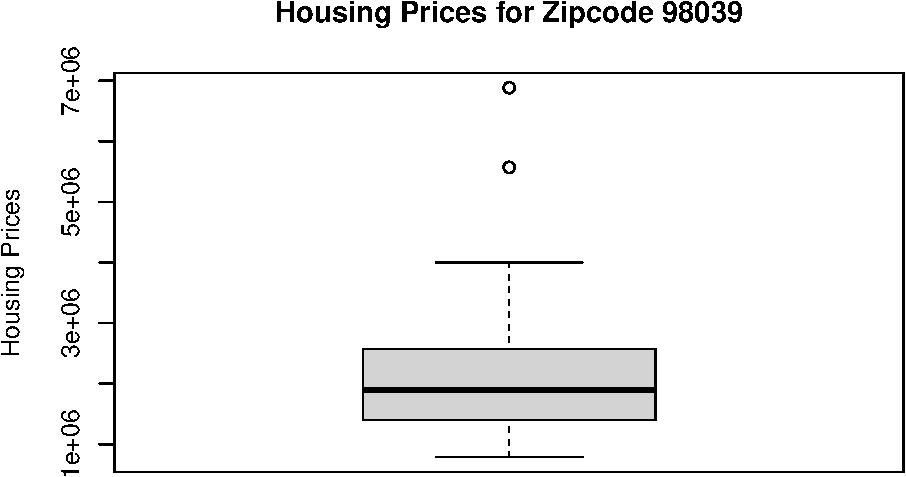
\includegraphics{HW2_Wu-Yulun_files/figure-latex/unnamed-chunk-1-1.pdf}

\begin{Shaded}
\begin{Highlighting}[]
\FunctionTok{boxplot}\NormalTok{(hp[}\FunctionTok{which}\NormalTok{(hp[}\StringTok{"zipcode"}\NormalTok{]}\SpecialCharTok{==}\FunctionTok{names}\NormalTok{(sort\_zip\_byavgprice[}\DecValTok{2}\NormalTok{])),}\StringTok{"price"}\NormalTok{],}\AttributeTok{main=}\StringTok{"Housing Prices for Zipcode 98004"}\NormalTok{,}\AttributeTok{ylab=}\StringTok{"Housing Prices"}\NormalTok{)}
\end{Highlighting}
\end{Shaded}

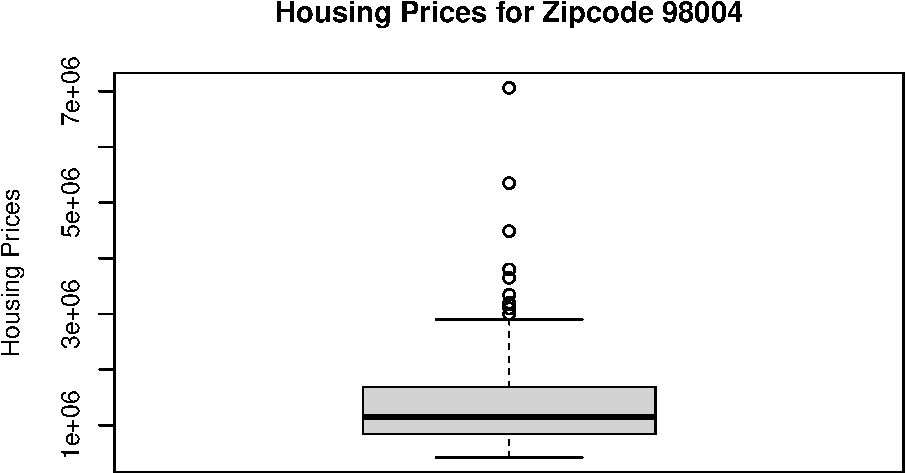
\includegraphics{HW2_Wu-Yulun_files/figure-latex/unnamed-chunk-1-2.pdf}

\begin{Shaded}
\begin{Highlighting}[]
\FunctionTok{boxplot}\NormalTok{(hp[}\FunctionTok{which}\NormalTok{(hp[}\StringTok{"zipcode"}\NormalTok{]}\SpecialCharTok{==}\FunctionTok{names}\NormalTok{(sort\_zip\_byavgprice[}\DecValTok{3}\NormalTok{])),}\StringTok{"price"}\NormalTok{],}\AttributeTok{main=}\StringTok{"Housing Prices for Zipcode 98040"}\NormalTok{,}\AttributeTok{ylab=}\StringTok{"Housing Prices"}\NormalTok{)}
\end{Highlighting}
\end{Shaded}

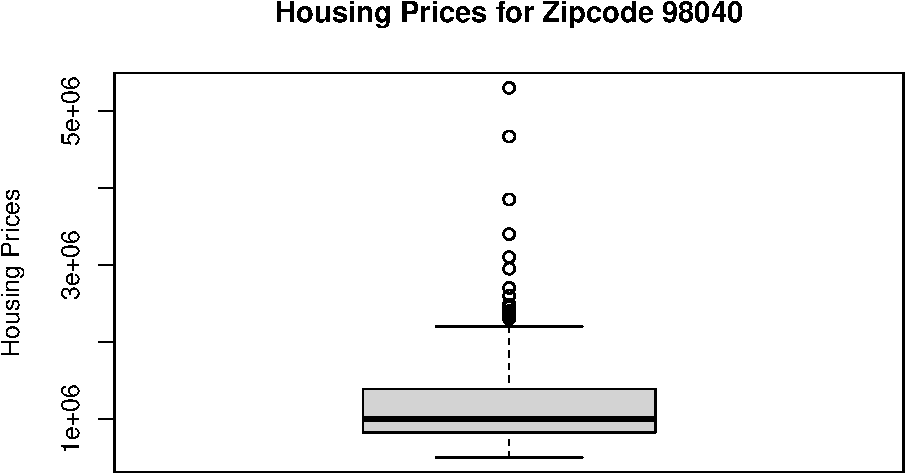
\includegraphics{HW2_Wu-Yulun_files/figure-latex/unnamed-chunk-1-3.pdf}

The top 3 zipcodes whose average housing prices are most expensive are:
98039, 98004, 98040 (listed in decreasing order of average housing
prices).

\begin{enumerate}
\def\labelenumi{(\alph{enumi})}
\setcounter{enumi}{1}
\tightlist
\item
\end{enumerate}

\begin{Shaded}
\begin{Highlighting}[]
\FunctionTok{plot}\NormalTok{(hp}\SpecialCharTok{$}\NormalTok{sqft\_living,hp}\SpecialCharTok{$}\NormalTok{price,}\AttributeTok{col=}\StringTok{"blue3"}\NormalTok{,}\AttributeTok{ylab=}\StringTok{"Housing Prices"}\NormalTok{,}\AttributeTok{xlab=}\StringTok{"Square Feet Living"}\NormalTok{,}\AttributeTok{main=}\StringTok{"Scatter Plot Of Square Feet Living And Housing Prices"}\NormalTok{)}
\end{Highlighting}
\end{Shaded}

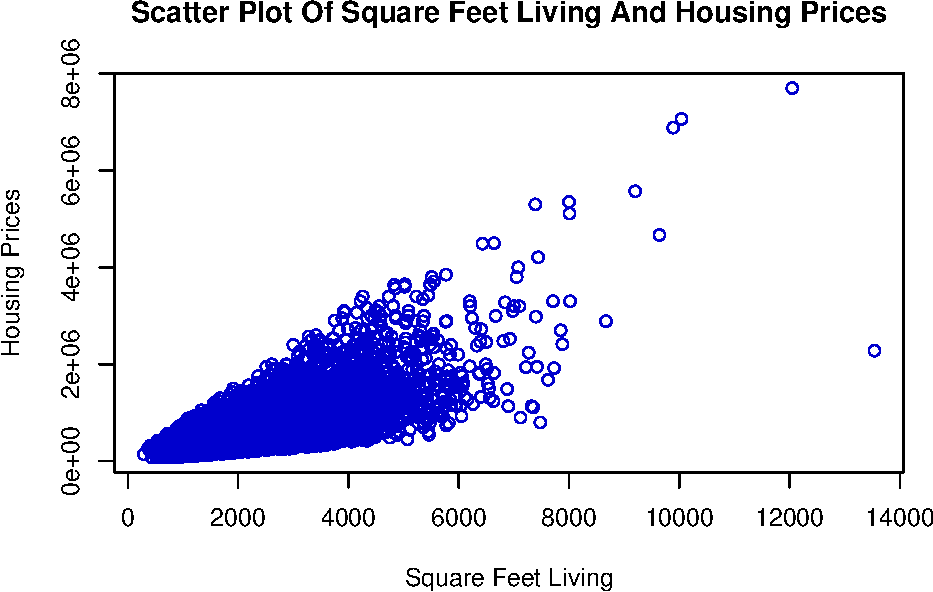
\includegraphics{HW2_Wu-Yulun_files/figure-latex/unnamed-chunk-2-1.pdf}

\begin{enumerate}
\def\labelenumi{(\alph{enumi})}
\setcounter{enumi}{2}
\tightlist
\item
\end{enumerate}

\begin{Shaded}
\begin{Highlighting}[]
\CommentTok{\# Read file of training and testing data}
\NormalTok{train\_data }\OtherTok{=} \FunctionTok{read.csv}\NormalTok{(}\StringTok{"train.data.csv"}\NormalTok{,}\AttributeTok{header =}\NormalTok{ T)}
\NormalTok{test\_data }\OtherTok{=} \FunctionTok{read.csv}\NormalTok{(}\StringTok{"test.data.csv"}\NormalTok{,}\AttributeTok{header =}\NormalTok{ T)}
\CommentTok{\# Fit linear model}
\NormalTok{model1 }\OtherTok{=} \FunctionTok{lm}\NormalTok{(price}\SpecialCharTok{\textasciitilde{}}\NormalTok{bedrooms}\SpecialCharTok{+}\NormalTok{bathrooms}\SpecialCharTok{+}\NormalTok{sqft\_living}\SpecialCharTok{+}\NormalTok{sqft\_lot,}\AttributeTok{data =}\NormalTok{ train\_data)}
\NormalTok{Ybar}\OtherTok{=}\FunctionTok{mean}\NormalTok{(test\_data[,}\StringTok{"price"}\NormalTok{])}
\NormalTok{SST}\OtherTok{=}\FunctionTok{sum}\NormalTok{((test\_data[,}\StringTok{"price"}\NormalTok{]}\SpecialCharTok{{-}}\NormalTok{Ybar)}\SpecialCharTok{\^{}}\DecValTok{2}\NormalTok{)}

\CommentTok{\# Calculate R\^{}2 for testing data}
\NormalTok{Yhat}\OtherTok{=}\FunctionTok{predict}\NormalTok{(model1,test\_data) }\CommentTok{\# Predicted Y}
\NormalTok{SSE}\OtherTok{=}\FunctionTok{sum}\NormalTok{((test\_data[,}\StringTok{"price"}\NormalTok{]}\SpecialCharTok{{-}}\NormalTok{Yhat)}\SpecialCharTok{\^{}}\DecValTok{2}\NormalTok{)}

\FunctionTok{cat}\NormalTok{(}\StringTok{"R\^{}2 on training data is"}\NormalTok{,}\FunctionTok{summary}\NormalTok{(model1)}\SpecialCharTok{$}\NormalTok{r.squared,}\StringTok{"}\SpecialCharTok{\textbackslash{}n}\StringTok{"}\NormalTok{)}
\end{Highlighting}
\end{Shaded}

\begin{verbatim}
## R^2 on training data is 0.5101139
\end{verbatim}

\begin{Shaded}
\begin{Highlighting}[]
\FunctionTok{cat}\NormalTok{(}\StringTok{"R\^{}2 on testing data is"}\NormalTok{,}\DecValTok{1}\SpecialCharTok{{-}}\NormalTok{(SSE}\SpecialCharTok{/}\NormalTok{SST),}\StringTok{"}\SpecialCharTok{\textbackslash{}n}\StringTok{"}\NormalTok{)}
\end{Highlighting}
\end{Shaded}

\begin{verbatim}
## R^2 on testing data is 0.5049945
\end{verbatim}

\(R^2\) of the model on training data is 0.5101139. \(R^2\) on testing
data is 0.5049945.

\begin{enumerate}
\def\labelenumi{(\alph{enumi})}
\setcounter{enumi}{3}
\tightlist
\item
\end{enumerate}

\begin{Shaded}
\begin{Highlighting}[]
\NormalTok{model2 }\OtherTok{=} \FunctionTok{update}\NormalTok{(model1, .}\SpecialCharTok{\textasciitilde{}}\NormalTok{. }\SpecialCharTok{+}\NormalTok{ zipcode)}
\CommentTok{\# Calculate R\^{}2 for testing data with model after adding zipcode}
\NormalTok{Ybar}\OtherTok{=}\FunctionTok{mean}\NormalTok{(test\_data[,}\StringTok{"price"}\NormalTok{])}
\NormalTok{SST}\OtherTok{=}\FunctionTok{sum}\NormalTok{((test\_data[,}\StringTok{"price"}\NormalTok{]}\SpecialCharTok{{-}}\NormalTok{Ybar)}\SpecialCharTok{\^{}}\DecValTok{2}\NormalTok{)}
\NormalTok{Yhat}\OtherTok{=}\FunctionTok{predict}\NormalTok{(model2,test\_data) }\CommentTok{\# Predicted Y}
\NormalTok{SSE}\OtherTok{=}\FunctionTok{sum}\NormalTok{((test\_data[,}\StringTok{"price"}\NormalTok{]}\SpecialCharTok{{-}}\NormalTok{Yhat)}\SpecialCharTok{\^{}}\DecValTok{2}\NormalTok{)}

\FunctionTok{cat}\NormalTok{(}\StringTok{"R\^{}2 on training data is"}\NormalTok{,}\FunctionTok{summary}\NormalTok{(model2)}\SpecialCharTok{$}\NormalTok{r.squared,}\StringTok{"}\SpecialCharTok{\textbackslash{}n}\StringTok{"}\NormalTok{)}
\end{Highlighting}
\end{Shaded}

\begin{verbatim}
## R^2 on training data is 0.5162971
\end{verbatim}

\begin{Shaded}
\begin{Highlighting}[]
\FunctionTok{cat}\NormalTok{(}\StringTok{"R\^{}2 on testing data is"}\NormalTok{,}\DecValTok{1}\SpecialCharTok{{-}}\NormalTok{(SSE}\SpecialCharTok{/}\NormalTok{SST),}\StringTok{"}\SpecialCharTok{\textbackslash{}n}\StringTok{"}\NormalTok{)}
\end{Highlighting}
\end{Shaded}

\begin{verbatim}
## R^2 on testing data is 0.5120097
\end{verbatim}

\(R^2\) of the model on training data after adding zipcode to linear
model is 0.5162971. \(R^2\) on testing data after adding zipcode to
linear model is 0.5120097.

\begin{enumerate}
\def\labelenumi{(\alph{enumi})}
\setcounter{enumi}{4}
\tightlist
\item
\end{enumerate}

\begin{Shaded}
\begin{Highlighting}[]
\CommentTok{\# Read file of training and testing data}
\NormalTok{fancyhouse }\OtherTok{=} \FunctionTok{read.csv}\NormalTok{(}\StringTok{"fancyhouse.csv"}\NormalTok{,}\AttributeTok{header =}\NormalTok{ T)}
\NormalTok{fancyhouse}
\end{Highlighting}
\end{Shaded}

\begin{verbatim}
##   X bedrooms bathrooms sqft_living sqft_lot floors zipcode condition grade
## 1 1        8        25       50000   225000      4   98039        10    10
##   waterfront view sqft_above sqft_basement yr_built yr_renovated      lat
## 1          1    4      37500         12500     1994         2010 47.62761
##        long sqft_living15 sqft_lot15
## 1 -122.2421          5000      40000
\end{verbatim}

\begin{Shaded}
\begin{Highlighting}[]
\NormalTok{price\_fancyhouse}\OtherTok{=}\FunctionTok{predict}\NormalTok{(model2,fancyhouse)}
\NormalTok{price\_fancyhouse}
\end{Highlighting}
\end{Shaded}

\begin{verbatim}
##        1 
## 15642273
\end{verbatim}

The predicted price for Bill Gates' house is 15642273. I don't think the
predicted price is reasonable, the real price probably is 10 times of
that, based on what I saw from luxury house tour on YouTube, the house
that has 5 bedrooms already worth more than this predicted price.

\begin{enumerate}
\def\labelenumi{(\alph{enumi})}
\setcounter{enumi}{5}
\tightlist
\item
\end{enumerate}

Since
\(R^2=1-\frac{SSE}{SST}=1-\frac{\sum_{i=1}^{n}(Y_i-X\widehat{\beta})^2}{\sum_{i=1}^{n}(Y_i-\bar{Y})^2}\).
SST remains unchanged no matter how \(X\widehat{\beta}\) changes, so the
only term that can change is
\(SSE=\sum_{i=1}^{n}(Y_i-X\widehat{\beta})^2\), and since
\(SSE=\sum_{i=1}^{n}(Y_i-X\widehat{\beta})^2 \propto ||Y-X\widehat{\beta}||_2^2\),
so we can compare \(R^2\) of model with d covariates and d+1 covariates
by comparing OLS. And model with smaller OLS will have bigger \(R^2\).
Further more, since Y remains unchanged, basically we are comparing
\(X\widehat{\beta}\) and \(X_1\widehat{\beta}_1\), the one closer to Y
will gives smaller OLS therefore bigger \(R^2\).

\(\because \widehat{\beta}=X(X'X)^{-1}X'Y\),\(\widehat{\beta}_1=X_1(X_1'X_1)^{-1}X_1'Y\)
and \(n>d+1\)

\(\therefore \widehat{\beta}\) is a d by 1 vector and
\(\widehat{\beta}_1\) is d+1 by 1 vector

\(\therefore\) We have chance to get a better approximation of Y by
\(X_1\widehat{\beta}_1\) compare to \(X\widehat{\beta}\) since we have
additional flexibility in \(\widehat{\beta}_1\) (ie: df of SSE with d+1
covariates is 1 greater than df of SSE with d covariates). Also \(R^2\)
can stay unchanged if \(\widehat{\beta}_{d+1}=0\) because basically
\(X\widehat{\beta}=X_1\widehat{\beta}_1\) in this case, so
\(SSE_{d+1}=SSE_d\) implies \(R^2_{d+1}=R^2_d\).

\(\therefore |Y-X_1\widehat{\beta}_1|\leq|Y-X\widehat{\beta}|\)

\(\therefore SSE_{d+1} \leq SSE_d\)

\(\therefore R^2_{d+1}\geq R^2_d\)

Thus, adding another covariate in the model never hurts \(R^2\) over the
training data.

\hypertarget{question-2-20-points-feature-engineering}{%
\subsection{Question 2 (20 Points) Feature
Engineering}\label{question-2-20-points-feature-engineering}}

\hypertarget{answer-1}{%
\subsubsection{Answer:}\label{answer-1}}

\begin{enumerate}
\def\labelenumi{(\alph{enumi})}
\tightlist
\item
\end{enumerate}

\begin{Shaded}
\begin{Highlighting}[]
\NormalTok{model3 }\OtherTok{=} \FunctionTok{update}\NormalTok{(model2, .}\SpecialCharTok{\textasciitilde{}}\NormalTok{. }\SpecialCharTok{+}\NormalTok{ bedrooms}\SpecialCharTok{*}\NormalTok{bathrooms)}
\CommentTok{\# Calculate R\^{}2 for testing data with model after adding bedrooms*bathrooms}
\NormalTok{Ybar}\OtherTok{=}\FunctionTok{mean}\NormalTok{(test\_data[,}\StringTok{"price"}\NormalTok{])}
\NormalTok{SST}\OtherTok{=}\FunctionTok{sum}\NormalTok{((test\_data[,}\StringTok{"price"}\NormalTok{]}\SpecialCharTok{{-}}\NormalTok{Ybar)}\SpecialCharTok{\^{}}\DecValTok{2}\NormalTok{)}
\NormalTok{Yhat}\OtherTok{=}\FunctionTok{predict}\NormalTok{(model3,test\_data) }\CommentTok{\# Predicted Y}
\NormalTok{SSE}\OtherTok{=}\FunctionTok{sum}\NormalTok{((test\_data[,}\StringTok{"price"}\NormalTok{]}\SpecialCharTok{{-}}\NormalTok{Yhat)}\SpecialCharTok{\^{}}\DecValTok{2}\NormalTok{)}

\FunctionTok{cat}\NormalTok{(}\StringTok{"R\^{}2 on training data is"}\NormalTok{,}\FunctionTok{summary}\NormalTok{(model3)}\SpecialCharTok{$}\NormalTok{r.squared,}\StringTok{"}\SpecialCharTok{\textbackslash{}n}\StringTok{"}\NormalTok{)}
\end{Highlighting}
\end{Shaded}

\begin{verbatim}
## R^2 on training data is 0.5223738
\end{verbatim}

\begin{Shaded}
\begin{Highlighting}[]
\FunctionTok{cat}\NormalTok{(}\StringTok{"R\^{}2 on testing data is"}\NormalTok{,}\DecValTok{1}\SpecialCharTok{{-}}\NormalTok{(SSE}\SpecialCharTok{/}\NormalTok{SST),}\StringTok{"}\SpecialCharTok{\textbackslash{}n}\StringTok{"}\NormalTok{)}
\end{Highlighting}
\end{Shaded}

\begin{verbatim}
## R^2 on testing data is 0.5165114
\end{verbatim}

\(R^2\) of the model with interaction of bedrooms and bathrooms added on
training data is 0.5223738. \(R^2\) of the model with interaction of
bedrooms and bathrooms added on testing data is 0.5165114.

\begin{enumerate}
\def\labelenumi{(\alph{enumi})}
\setcounter{enumi}{1}
\tightlist
\item
\end{enumerate}

\begin{Shaded}
\begin{Highlighting}[]
\NormalTok{model4 }\OtherTok{=} \FunctionTok{update}\NormalTok{(model3, .}\SpecialCharTok{\textasciitilde{}}\NormalTok{. }\SpecialCharTok{+}\NormalTok{ bathrooms}\SpecialCharTok{*}\NormalTok{sqft\_living)}
\CommentTok{\# Calculate R\^{}2 for testing data with model after adding bathrooms*sqft\_living}
\NormalTok{Ybar}\OtherTok{=}\FunctionTok{mean}\NormalTok{(test\_data[,}\StringTok{"price"}\NormalTok{])}
\NormalTok{SST}\OtherTok{=}\FunctionTok{sum}\NormalTok{((test\_data[,}\StringTok{"price"}\NormalTok{]}\SpecialCharTok{{-}}\NormalTok{Ybar)}\SpecialCharTok{\^{}}\DecValTok{2}\NormalTok{)}
\NormalTok{Yhat}\OtherTok{=}\FunctionTok{predict}\NormalTok{(model4,test\_data) }\CommentTok{\# Predicted Y}
\NormalTok{SSE}\OtherTok{=}\FunctionTok{sum}\NormalTok{((test\_data[,}\StringTok{"price"}\NormalTok{]}\SpecialCharTok{{-}}\NormalTok{Yhat)}\SpecialCharTok{\^{}}\DecValTok{2}\NormalTok{)}

\FunctionTok{cat}\NormalTok{(}\StringTok{"R\^{}2 on training data is"}\NormalTok{,}\FunctionTok{summary}\NormalTok{(model4)}\SpecialCharTok{$}\NormalTok{r.squared,}\StringTok{"}\SpecialCharTok{\textbackslash{}n}\StringTok{"}\NormalTok{)}
\end{Highlighting}
\end{Shaded}

\begin{verbatim}
## R^2 on training data is 0.5490765
\end{verbatim}

\begin{Shaded}
\begin{Highlighting}[]
\FunctionTok{cat}\NormalTok{(}\StringTok{"R\^{}2 on testing data is"}\NormalTok{,}\DecValTok{1}\SpecialCharTok{{-}}\NormalTok{(SSE}\SpecialCharTok{/}\NormalTok{SST),}\StringTok{"}\SpecialCharTok{\textbackslash{}n}\StringTok{"}\NormalTok{)}
\end{Highlighting}
\end{Shaded}

\begin{verbatim}
## R^2 on testing data is 0.5451303
\end{verbatim}

\(R^2\) of the model with interaction of sqft\_living and bathrooms
added on testing data is 0.5451303.

\begin{enumerate}
\def\labelenumi{(\alph{enumi})}
\setcounter{enumi}{2}
\tightlist
\item
\end{enumerate}

\begin{Shaded}
\begin{Highlighting}[]
\NormalTok{model5 }\OtherTok{=} \FunctionTok{update}\NormalTok{(model2, .}\SpecialCharTok{\textasciitilde{}}\NormalTok{. }\SpecialCharTok{+} \FunctionTok{poly}\NormalTok{(bedrooms, }\DecValTok{3}\NormalTok{)}\SpecialCharTok{+} \FunctionTok{poly}\NormalTok{(bathrooms, }\DecValTok{3}\NormalTok{))}
\CommentTok{\# Calculate R\^{}2 for testing data with model after adding bedrooms*bathrooms}
\NormalTok{Ybar}\OtherTok{=}\FunctionTok{mean}\NormalTok{(test\_data[,}\StringTok{"price"}\NormalTok{])}
\NormalTok{SST}\OtherTok{=}\FunctionTok{sum}\NormalTok{((test\_data[,}\StringTok{"price"}\NormalTok{]}\SpecialCharTok{{-}}\NormalTok{Ybar)}\SpecialCharTok{\^{}}\DecValTok{2}\NormalTok{)}
\NormalTok{Yhat}\OtherTok{=}\FunctionTok{predict}\NormalTok{(model5,test\_data) }\CommentTok{\# Predicted Y}
\NormalTok{SSE}\OtherTok{=}\FunctionTok{sum}\NormalTok{((test\_data[,}\StringTok{"price"}\NormalTok{]}\SpecialCharTok{{-}}\NormalTok{Yhat)}\SpecialCharTok{\^{}}\DecValTok{2}\NormalTok{)}

\FunctionTok{cat}\NormalTok{(}\StringTok{"R\^{}2 on training data is"}\NormalTok{,}\FunctionTok{summary}\NormalTok{(model5)}\SpecialCharTok{$}\NormalTok{r.squared,}\StringTok{"}\SpecialCharTok{\textbackslash{}n}\StringTok{"}\NormalTok{)}
\end{Highlighting}
\end{Shaded}

\begin{verbatim}
## R^2 on training data is 0.5424973
\end{verbatim}

\begin{Shaded}
\begin{Highlighting}[]
\FunctionTok{cat}\NormalTok{(}\StringTok{"R\^{}2 on testing data is"}\NormalTok{,}\DecValTok{1}\SpecialCharTok{{-}}\NormalTok{(SSE}\SpecialCharTok{/}\NormalTok{SST),}\StringTok{"}\SpecialCharTok{\textbackslash{}n}\StringTok{"}\NormalTok{)}
\end{Highlighting}
\end{Shaded}

\begin{verbatim}
## R^2 on testing data is 0.5285074
\end{verbatim}

\(R^2\) of the model with polynomial term with degree 2 and 3 of
bedrooms and bathrooms added on training data is 0.5424973. \(R^2\) of
the model with polynomial term with degree 2 and 3 of bedrooms and
bathrooms added on testing data is 0.5285074.

\hypertarget{question-3-20-points-wine-pricing}{%
\subsection{Question 3 (20 Points) Wine
Pricing}\label{question-3-20-points-wine-pricing}}

\hypertarget{answer-2}{%
\subsubsection{Answer:}\label{answer-2}}

Part I

\begin{Shaded}
\begin{Highlighting}[]
\CommentTok{\# Read file of wine data}
\NormalTok{wine }\OtherTok{=} \FunctionTok{read.csv}\NormalTok{(}\StringTok{"wine.csv"}\NormalTok{,}\AttributeTok{header =}\NormalTok{ T)}
\CommentTok{\# 4 Scatter plots}
\FunctionTok{plot}\NormalTok{(wine}\SpecialCharTok{$}\NormalTok{AGST,wine}\SpecialCharTok{$}\NormalTok{Price,}\AttributeTok{main=}\StringTok{"Wine Price v.s. Average}
\StringTok{Growing Season Temperature(AGST)"}\NormalTok{,}\AttributeTok{ylab=}\StringTok{"Wine Price"}\NormalTok{,}\AttributeTok{xlab=}\StringTok{"Average}
\StringTok{Growing Season Temperature(AGST)"}\NormalTok{)}
\end{Highlighting}
\end{Shaded}

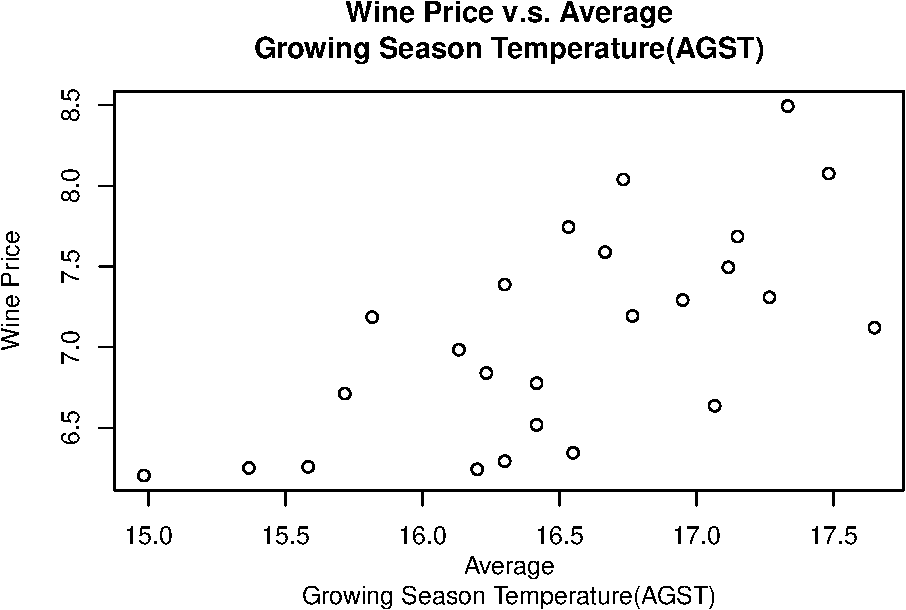
\includegraphics{HW2_Wu-Yulun_files/figure-latex/unnamed-chunk-9-1.pdf}

\begin{Shaded}
\begin{Highlighting}[]
\FunctionTok{plot}\NormalTok{(wine}\SpecialCharTok{$}\NormalTok{WinterRain,wine}\SpecialCharTok{$}\NormalTok{Price,}\AttributeTok{main=}\StringTok{"Wine Price v.s. Winter Rain Amount"}\NormalTok{,}\AttributeTok{ylab=}\StringTok{"Wine Price"}\NormalTok{,}\AttributeTok{xlab=}\StringTok{"Winter Rain Amount"}\NormalTok{)}
\end{Highlighting}
\end{Shaded}

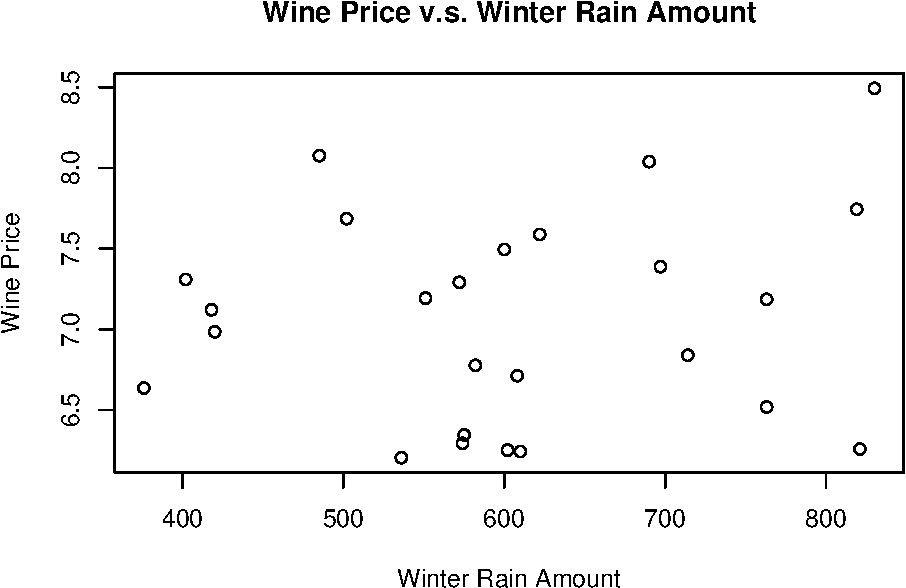
\includegraphics{HW2_Wu-Yulun_files/figure-latex/unnamed-chunk-9-2.pdf}

\begin{Shaded}
\begin{Highlighting}[]
\FunctionTok{plot}\NormalTok{(wine}\SpecialCharTok{$}\NormalTok{HarvestRain,wine}\SpecialCharTok{$}\NormalTok{Price,}\AttributeTok{main=}\StringTok{"Wine Price v.s. Harvest Rain Amount"}\NormalTok{,}\AttributeTok{ylab=}\StringTok{"Wine Price"}\NormalTok{,}\AttributeTok{xlab=}\StringTok{"Harvest Rain Amount"}\NormalTok{)}
\end{Highlighting}
\end{Shaded}

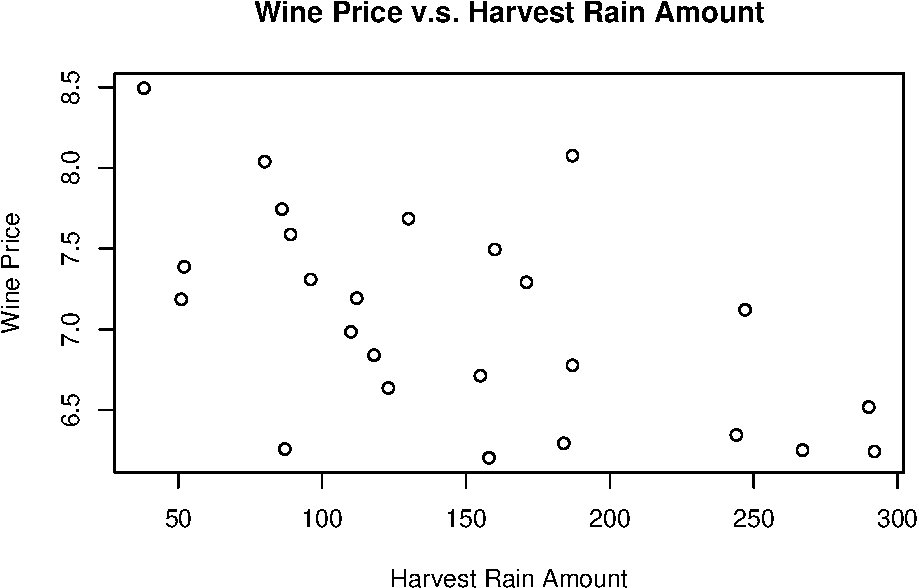
\includegraphics{HW2_Wu-Yulun_files/figure-latex/unnamed-chunk-9-3.pdf}

\begin{Shaded}
\begin{Highlighting}[]
\FunctionTok{plot}\NormalTok{(wine}\SpecialCharTok{$}\NormalTok{Age,wine}\SpecialCharTok{$}\NormalTok{Price,}\AttributeTok{main=}\StringTok{"Wine Price v.s. Age Of Wine"}\NormalTok{,}\AttributeTok{ylab=}\StringTok{"Wine Price"}\NormalTok{,}\AttributeTok{xlab=}\StringTok{"Age Of Wine"}\NormalTok{)}
\end{Highlighting}
\end{Shaded}

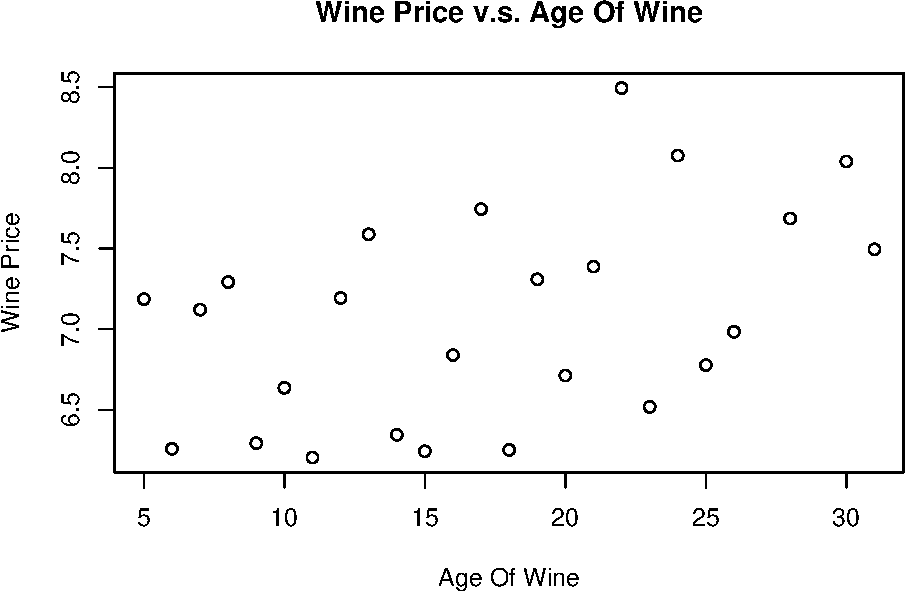
\includegraphics{HW2_Wu-Yulun_files/figure-latex/unnamed-chunk-9-4.pdf}

\begin{Shaded}
\begin{Highlighting}[]
\NormalTok{mean\_price }\OtherTok{=} \FunctionTok{mean}\NormalTok{(wine[,}\StringTok{"Price"}\NormalTok{]) }\CommentTok{\# ybar}
\NormalTok{mean\_AGST }\OtherTok{=} \FunctionTok{mean}\NormalTok{(wine[,}\StringTok{"AGST"}\NormalTok{]) }\CommentTok{\# mean of AGST}
\NormalTok{mean\_WinterRain }\OtherTok{=} \FunctionTok{mean}\NormalTok{(wine[,}\StringTok{"WinterRain"}\NormalTok{]) }\CommentTok{\# mean of WinterRain}
\NormalTok{mean\_HarvestRain }\OtherTok{=} \FunctionTok{mean}\NormalTok{(wine[,}\StringTok{"HarvestRain"}\NormalTok{]) }\CommentTok{\# mean of HarvestRain}
\NormalTok{mean\_Age }\OtherTok{=} \FunctionTok{mean}\NormalTok{(wine[,}\StringTok{"Age"}\NormalTok{]) }\CommentTok{\# mean of Age}

\NormalTok{rAGST }\OtherTok{=} \FunctionTok{sum}\NormalTok{((wine[,}\StringTok{"AGST"}\NormalTok{]}\SpecialCharTok{{-}}\NormalTok{mean\_AGST)}\SpecialCharTok{*}\NormalTok{(wine[,}\StringTok{"Price"}\NormalTok{]}\SpecialCharTok{{-}}\NormalTok{mean\_price))}\SpecialCharTok{/}\FunctionTok{sqrt}\NormalTok{(}\FunctionTok{sum}\NormalTok{((wine[,}\StringTok{"AGST"}\NormalTok{]}\SpecialCharTok{{-}}\NormalTok{mean\_AGST)}\SpecialCharTok{\^{}}\DecValTok{2}\NormalTok{)}\SpecialCharTok{*}\FunctionTok{sum}\NormalTok{((wine[,}\StringTok{"Price"}\NormalTok{]}\SpecialCharTok{{-}}\NormalTok{mean\_price)}\SpecialCharTok{\^{}}\DecValTok{2}\NormalTok{)) }\CommentTok{\# Pearson Cor Price and AGST}
\NormalTok{rAGST}
\end{Highlighting}
\end{Shaded}

\begin{verbatim}
## [1] 0.6595629
\end{verbatim}

\begin{Shaded}
\begin{Highlighting}[]
\NormalTok{rWinterRain }\OtherTok{=} \FunctionTok{sum}\NormalTok{((wine[,}\StringTok{"WinterRain"}\NormalTok{]}\SpecialCharTok{{-}}\NormalTok{mean\_WinterRain)}\SpecialCharTok{*}\NormalTok{(wine[,}\StringTok{"Price"}\NormalTok{]}\SpecialCharTok{{-}}\NormalTok{mean\_price))}\SpecialCharTok{/}\FunctionTok{sqrt}\NormalTok{(}\FunctionTok{sum}\NormalTok{((wine[,}\StringTok{"WinterRain"}\NormalTok{]}\SpecialCharTok{{-}}\NormalTok{mean\_WinterRain)}\SpecialCharTok{\^{}}\DecValTok{2}\NormalTok{)}\SpecialCharTok{*}\FunctionTok{sum}\NormalTok{((wine[,}\StringTok{"Price"}\NormalTok{]}\SpecialCharTok{{-}}\NormalTok{mean\_price)}\SpecialCharTok{\^{}}\DecValTok{2}\NormalTok{)) }\CommentTok{\# Pearson Cor Price and WinterRain}
\NormalTok{rWinterRain}
\end{Highlighting}
\end{Shaded}

\begin{verbatim}
## [1] 0.1366505
\end{verbatim}

\begin{Shaded}
\begin{Highlighting}[]
\NormalTok{rHarvestRain }\OtherTok{=} \FunctionTok{sum}\NormalTok{((wine[,}\StringTok{"HarvestRain"}\NormalTok{]}\SpecialCharTok{{-}}\NormalTok{mean\_HarvestRain)}\SpecialCharTok{*}\NormalTok{(wine[,}\StringTok{"Price"}\NormalTok{]}\SpecialCharTok{{-}}\NormalTok{mean\_price))}\SpecialCharTok{/}\FunctionTok{sqrt}\NormalTok{(}\FunctionTok{sum}\NormalTok{((wine[,}\StringTok{"HarvestRain"}\NormalTok{]}\SpecialCharTok{{-}}\NormalTok{mean\_HarvestRain)}\SpecialCharTok{\^{}}\DecValTok{2}\NormalTok{)}\SpecialCharTok{*}\FunctionTok{sum}\NormalTok{((wine[,}\StringTok{"Price"}\NormalTok{]}\SpecialCharTok{{-}}\NormalTok{mean\_price)}\SpecialCharTok{\^{}}\DecValTok{2}\NormalTok{)) }\CommentTok{\# Pearson Cor Price and HarvestRain}
\NormalTok{rHarvestRain}
\end{Highlighting}
\end{Shaded}

\begin{verbatim}
## [1] -0.5633219
\end{verbatim}

\begin{Shaded}
\begin{Highlighting}[]
\NormalTok{rAge }\OtherTok{=} \FunctionTok{sum}\NormalTok{((wine[,}\StringTok{"Age"}\NormalTok{]}\SpecialCharTok{{-}}\NormalTok{mean\_Age)}\SpecialCharTok{*}\NormalTok{(wine[,}\StringTok{"Price"}\NormalTok{]}\SpecialCharTok{{-}}\NormalTok{mean\_price))}\SpecialCharTok{/}\FunctionTok{sqrt}\NormalTok{(}\FunctionTok{sum}\NormalTok{((wine[,}\StringTok{"Age"}\NormalTok{]}\SpecialCharTok{{-}}\NormalTok{mean\_Age)}\SpecialCharTok{\^{}}\DecValTok{2}\NormalTok{)}\SpecialCharTok{*}\FunctionTok{sum}\NormalTok{((wine[,}\StringTok{"Price"}\NormalTok{]}\SpecialCharTok{{-}}\NormalTok{mean\_price)}\SpecialCharTok{\^{}}\DecValTok{2}\NormalTok{)) }\CommentTok{\# Pearson Cor Price and Age}
\NormalTok{rAge}
\end{Highlighting}
\end{Shaded}

\begin{verbatim}
## [1] 0.4477679
\end{verbatim}

Based on the scatter plot and Pearson's correlation calculated, average
growing season temperature (AGST) is most correlated with Price, their
Pearson's correlation is 0.6595629.

Part II

\begin{Shaded}
\begin{Highlighting}[]
\NormalTok{model1 }\OtherTok{=} \FunctionTok{lm}\NormalTok{(Price}\SpecialCharTok{\textasciitilde{}}\NormalTok{AGST,}\AttributeTok{data=}\NormalTok{wine)}
\FunctionTok{cat}\NormalTok{(}\StringTok{"Fitted coefficient of model Price\textasciitilde{}AGST is"}\NormalTok{,}\FunctionTok{summary}\NormalTok{(model1)}\SpecialCharTok{$}\NormalTok{coef[}\DecValTok{1}\NormalTok{],}\StringTok{","}\NormalTok{, }\FunctionTok{summary}\NormalTok{(model1)}\SpecialCharTok{$}\NormalTok{coef[}\DecValTok{2}\NormalTok{],}\StringTok{"}\SpecialCharTok{\textbackslash{}n}\StringTok{"}\NormalTok{)}
\end{Highlighting}
\end{Shaded}

\begin{verbatim}
## Fitted coefficient of model Price~AGST is -3.417761 , 0.6350943
\end{verbatim}

\begin{Shaded}
\begin{Highlighting}[]
\FunctionTok{cat}\NormalTok{(}\StringTok{"R\^{}2 of marginal model of Price\textasciitilde{}AGST is"}\NormalTok{,}\FunctionTok{summary}\NormalTok{(model1)}\SpecialCharTok{$}\NormalTok{r.squared,}\StringTok{"}\SpecialCharTok{\textbackslash{}n}\StringTok{"}\NormalTok{)}
\end{Highlighting}
\end{Shaded}

\begin{verbatim}
## R^2 of marginal model of Price~AGST is 0.4350232
\end{verbatim}

The fitted coefficient values for Price\textasciitilde AGST is
\[\beta_0=-3.4177613\] and \[\beta_1=0.6350943\]. \(R^2\) is 0.4350232.

Part III

\begin{Shaded}
\begin{Highlighting}[]
\CommentTok{\# Read file of winetest data}
\NormalTok{winetest }\OtherTok{=} \FunctionTok{read.csv}\NormalTok{(}\StringTok{"winetest.csv"}\NormalTok{,}\AttributeTok{header =}\NormalTok{ T)}

\NormalTok{Ybar }\OtherTok{=} \FunctionTok{mean}\NormalTok{(winetest}\SpecialCharTok{$}\NormalTok{Price)}
\NormalTok{SST }\OtherTok{=} \FunctionTok{sum}\NormalTok{((winetest}\SpecialCharTok{$}\NormalTok{Price}\SpecialCharTok{{-}}\NormalTok{Ybar)}\SpecialCharTok{\^{}}\DecValTok{2}\NormalTok{)}

\NormalTok{model2 }\OtherTok{=} \FunctionTok{update}\NormalTok{(model1, .}\SpecialCharTok{\textasciitilde{}}\NormalTok{. }\SpecialCharTok{+}\NormalTok{ HarvestRain) }\CommentTok{\# Add HarvestRain}
\FunctionTok{cat}\NormalTok{(}\StringTok{"R\^{}2 for training data after adding HarvestRain:"}\NormalTok{,}\FunctionTok{summary}\NormalTok{(model2)}\SpecialCharTok{$}\NormalTok{r.squared,}\StringTok{"}\SpecialCharTok{\textbackslash{}n}\StringTok{"}\NormalTok{)}
\end{Highlighting}
\end{Shaded}

\begin{verbatim}
## R^2 for training data after adding HarvestRain: 0.7073708
\end{verbatim}

\begin{Shaded}
\begin{Highlighting}[]
\CommentTok{\# Calculate R\^{}2 for testing data with model after adding HarvestRain}
\NormalTok{Yhat2}\OtherTok{=}\FunctionTok{predict}\NormalTok{(model2,winetest) }\CommentTok{\# Predicted Y}
\NormalTok{SSE }\OtherTok{=} \FunctionTok{sum}\NormalTok{((winetest}\SpecialCharTok{$}\NormalTok{Price}\SpecialCharTok{{-}}\NormalTok{Yhat2)}\SpecialCharTok{\^{}}\DecValTok{2}\NormalTok{)}
\FunctionTok{cat}\NormalTok{(}\StringTok{"R\^{}2 for testing data with model after adding HarvestRain:"}\NormalTok{,}\DecValTok{1}\SpecialCharTok{{-}}\NormalTok{(SSE}\SpecialCharTok{/}\NormalTok{SST),}\StringTok{"}\SpecialCharTok{\textbackslash{}n}\StringTok{"}\NormalTok{)}
\end{Highlighting}
\end{Shaded}

\begin{verbatim}
## R^2 for testing data with model after adding HarvestRain: -2.503339
\end{verbatim}

\begin{Shaded}
\begin{Highlighting}[]
\NormalTok{model3 }\OtherTok{=} \FunctionTok{update}\NormalTok{(model2, .}\SpecialCharTok{\textasciitilde{}}\NormalTok{. }\SpecialCharTok{+}\NormalTok{ Age) }\CommentTok{\# Add Age}
\FunctionTok{summary}\NormalTok{(model3)}\SpecialCharTok{$}\NormalTok{r.squared }\CommentTok{\# R\^{}2 for training data after adding Age}
\end{Highlighting}
\end{Shaded}

\begin{verbatim}
## [1] 0.7900362
\end{verbatim}

\begin{Shaded}
\begin{Highlighting}[]
\FunctionTok{cat}\NormalTok{(}\StringTok{"R\^{}2 for training data after adding Age:"}\NormalTok{,}\FunctionTok{summary}\NormalTok{(model3)}\SpecialCharTok{$}\NormalTok{r.squared,}\StringTok{"}\SpecialCharTok{\textbackslash{}n}\StringTok{"}\NormalTok{)}
\end{Highlighting}
\end{Shaded}

\begin{verbatim}
## R^2 for training data after adding Age: 0.7900362
\end{verbatim}

\begin{Shaded}
\begin{Highlighting}[]
\CommentTok{\# Calculate R\^{}2 for testing data with model after adding Age}
\NormalTok{Yhat3}\OtherTok{=}\FunctionTok{predict}\NormalTok{(model3,winetest) }\CommentTok{\# Predicted Y}
\NormalTok{SSE }\OtherTok{=} \FunctionTok{sum}\NormalTok{((winetest}\SpecialCharTok{$}\NormalTok{Price}\SpecialCharTok{{-}}\NormalTok{Yhat3)}\SpecialCharTok{\^{}}\DecValTok{2}\NormalTok{)}
\FunctionTok{cat}\NormalTok{(}\StringTok{"R\^{}2 for testing data with model after adding Age:"}\NormalTok{,}\DecValTok{1}\SpecialCharTok{{-}}\NormalTok{(SSE}\SpecialCharTok{/}\NormalTok{SST),}\StringTok{"}\SpecialCharTok{\textbackslash{}n}\StringTok{"}\NormalTok{)}
\end{Highlighting}
\end{Shaded}

\begin{verbatim}
## R^2 for testing data with model after adding Age: -0.5080824
\end{verbatim}

\begin{Shaded}
\begin{Highlighting}[]
\NormalTok{model4 }\OtherTok{=} \FunctionTok{update}\NormalTok{(model3, .}\SpecialCharTok{\textasciitilde{}}\NormalTok{. }\SpecialCharTok{+}\NormalTok{ WinterRain) }\CommentTok{\# Add WinterRain}
\FunctionTok{summary}\NormalTok{(model4)}\SpecialCharTok{$}\NormalTok{r.squared }\CommentTok{\# R\^{}2 for training data after adding WinterRain}
\end{Highlighting}
\end{Shaded}

\begin{verbatim}
## [1] 0.8285662
\end{verbatim}

\begin{Shaded}
\begin{Highlighting}[]
\FunctionTok{cat}\NormalTok{(}\StringTok{"R\^{}2 for training data after adding WinterRain:"}\NormalTok{,}\FunctionTok{summary}\NormalTok{(model4)}\SpecialCharTok{$}\NormalTok{r.squared,}\StringTok{"}\SpecialCharTok{\textbackslash{}n}\StringTok{"}\NormalTok{)}
\end{Highlighting}
\end{Shaded}

\begin{verbatim}
## R^2 for training data after adding WinterRain: 0.8285662
\end{verbatim}

\begin{Shaded}
\begin{Highlighting}[]
\CommentTok{\# Calculate R\^{}2 for testing data with model after adding WinterRain}
\NormalTok{Yhat4}\OtherTok{=}\FunctionTok{predict}\NormalTok{(model4,winetest) }\CommentTok{\# Predicted Y}
\NormalTok{SSE }\OtherTok{=} \FunctionTok{sum}\NormalTok{((winetest}\SpecialCharTok{$}\NormalTok{Price}\SpecialCharTok{{-}}\NormalTok{Yhat4)}\SpecialCharTok{\^{}}\DecValTok{2}\NormalTok{)}
\FunctionTok{cat}\NormalTok{(}\StringTok{"R\^{}2 for testing data with model after adding WinterRain:"}\NormalTok{,}\DecValTok{1}\SpecialCharTok{{-}}\NormalTok{(SSE}\SpecialCharTok{/}\NormalTok{SST),}\StringTok{"}\SpecialCharTok{\textbackslash{}n}\StringTok{"}\NormalTok{)}
\end{Highlighting}
\end{Shaded}

\begin{verbatim}
## R^2 for testing data with model after adding WinterRain: 0.3343905
\end{verbatim}

\begin{Shaded}
\begin{Highlighting}[]
\NormalTok{model5 }\OtherTok{=} \FunctionTok{update}\NormalTok{(model4, .}\SpecialCharTok{\textasciitilde{}}\NormalTok{. }\SpecialCharTok{+}\NormalTok{ FrancePop) }\CommentTok{\# Add FrancePop}
\FunctionTok{summary}\NormalTok{(model5)}\SpecialCharTok{$}\NormalTok{r.squared }\CommentTok{\# R\^{}2 for training data after adding FrancePop}
\end{Highlighting}
\end{Shaded}

\begin{verbatim}
## [1] 0.8293592
\end{verbatim}

\begin{Shaded}
\begin{Highlighting}[]
\FunctionTok{cat}\NormalTok{(}\StringTok{"R\^{}2 for training data after adding FrancePop:"}\NormalTok{,}\FunctionTok{summary}\NormalTok{(model5)}\SpecialCharTok{$}\NormalTok{r.squared,}\StringTok{"}\SpecialCharTok{\textbackslash{}n}\StringTok{"}\NormalTok{)}
\end{Highlighting}
\end{Shaded}

\begin{verbatim}
## R^2 for training data after adding FrancePop: 0.8293592
\end{verbatim}

\begin{Shaded}
\begin{Highlighting}[]
\CommentTok{\# Calculate R\^{}2 for testing data with model after adding FrancePop}
\NormalTok{Yhat5}\OtherTok{=}\FunctionTok{predict}\NormalTok{(model5,winetest) }\CommentTok{\# Predicted Y}
\NormalTok{SSE }\OtherTok{=} \FunctionTok{sum}\NormalTok{((winetest}\SpecialCharTok{$}\NormalTok{Price}\SpecialCharTok{{-}}\NormalTok{Yhat5)}\SpecialCharTok{\^{}}\DecValTok{2}\NormalTok{)}
\FunctionTok{cat}\NormalTok{(}\StringTok{"R\^{}2 for testing data with model after adding FrancePop:"}\NormalTok{,}\DecValTok{1}\SpecialCharTok{{-}}\NormalTok{(SSE}\SpecialCharTok{/}\NormalTok{SST),}\StringTok{"}\SpecialCharTok{\textbackslash{}n}\StringTok{"}\NormalTok{)}
\end{Highlighting}
\end{Shaded}

\begin{verbatim}
## R^2 for testing data with model after adding FrancePop: 0.2120672
\end{verbatim}

\begin{Shaded}
\begin{Highlighting}[]
\FunctionTok{summary}\NormalTok{(model4)}\SpecialCharTok{$}\NormalTok{coef}
\end{Highlighting}
\end{Shaded}

\begin{verbatim}
##                 Estimate   Std. Error   t value     Pr(>|t|)
## (Intercept) -3.429980187 1.7658975180 -1.942344 6.631093e-02
## AGST         0.607209348 0.0987022158  6.151932 5.197012e-06
## HarvestRain -0.003971534 0.0008537981 -4.651608 1.537556e-04
## Age          0.023930832 0.0080968750  2.955564 7.818874e-03
## WinterRain   0.001075505 0.0005072784  2.120148 4.669359e-02
\end{verbatim}

Based on testing \(R^2\), we should choose model of
Price\textasciitilde AGST+HarvestRain+Age+WinterRain. Since
\(\widehat{\beta}_{HarvestRain}\) is negative, so more rain in harvest
season will reduce the wine price. Since \(\widehat{\beta}_{AGST}\),
\(\widehat{\beta}_{Age}\), \(\widehat{\beta}_{WinterRain}\) are
positive, so higher average growing season temperature (AGST) and/or
older age and/or more rain in winter season will increase the wine
price. The interpretation of my model agree with Prof.~Ashenfelter's
finding.

\hypertarget{question-4-30-points-moneyball-the-analytics-edge-in-sports}{%
\subsection{Question 4 (30 Points) Moneyball: The Analytics Edge in
Sports}\label{question-4-30-points-moneyball-the-analytics-edge-in-sports}}

\hypertarget{answer-3}{%
\subsubsection{Answer:}\label{answer-3}}

Part I

\begin{Shaded}
\begin{Highlighting}[]
\CommentTok{\# Read file of baseball data}
\NormalTok{baseball }\OtherTok{=} \FunctionTok{read.csv}\NormalTok{(}\StringTok{"baseball.csv"}\NormalTok{,}\AttributeTok{header =}\NormalTok{ T)}

\CommentTok{\# Histogram and Boxplot of OBP}
\FunctionTok{par}\NormalTok{(}\AttributeTok{mfrow=}\FunctionTok{c}\NormalTok{(}\DecValTok{1}\NormalTok{,}\DecValTok{2}\NormalTok{))}
\FunctionTok{hist}\NormalTok{(baseball}\SpecialCharTok{$}\NormalTok{OBP,}\AttributeTok{main=}\StringTok{"Histogram Of On{-}Base Percentage (OBP)"}\NormalTok{,}\AttributeTok{xlab=}\StringTok{"On{-}Base Percentage (OBP)"}\NormalTok{)}
\FunctionTok{boxplot}\NormalTok{(baseball}\SpecialCharTok{$}\NormalTok{OBP,}\AttributeTok{main=}\StringTok{"Boxplot Of On{-}Base Percentage (OBP)"}\NormalTok{)}
\end{Highlighting}
\end{Shaded}

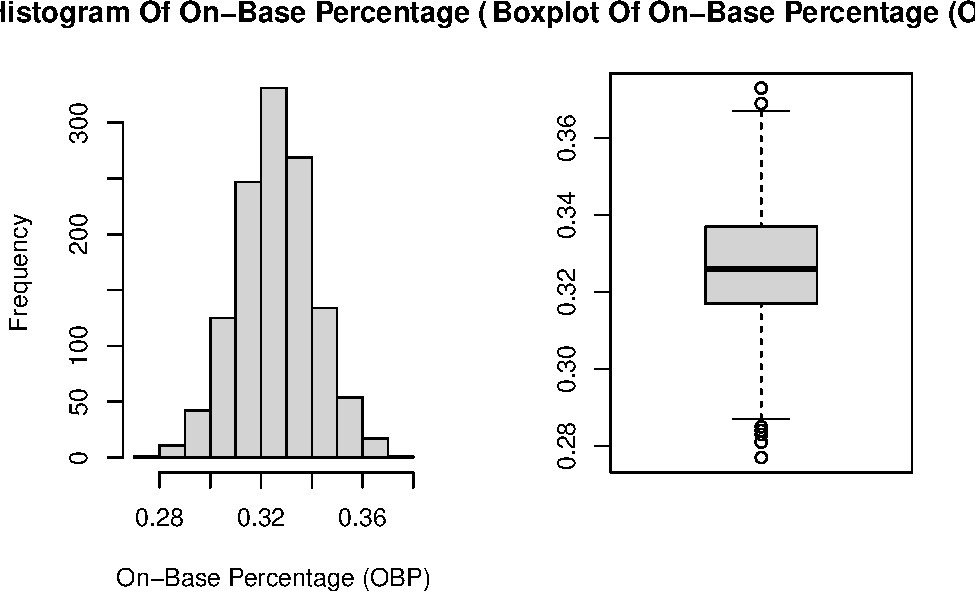
\includegraphics{HW2_Wu-Yulun_files/figure-latex/unnamed-chunk-12-1.pdf}

\begin{Shaded}
\begin{Highlighting}[]
\NormalTok{mean\_OBP }\OtherTok{=} \FunctionTok{mean}\NormalTok{(baseball}\SpecialCharTok{$}\NormalTok{OBP) }\CommentTok{\# Mean of OBP}
\FunctionTok{cat}\NormalTok{(}\StringTok{"The mean of OBP:"}\NormalTok{,mean\_OBP,}\StringTok{"}\SpecialCharTok{\textbackslash{}n}\StringTok{"}\NormalTok{)}
\end{Highlighting}
\end{Shaded}

\begin{verbatim}
## The mean of OBP: 0.3263312
\end{verbatim}

\begin{Shaded}
\begin{Highlighting}[]
\NormalTok{median\_OBP }\OtherTok{=} \FunctionTok{median}\NormalTok{(baseball}\SpecialCharTok{$}\NormalTok{OBP) }\CommentTok{\# Median of OBP}
\FunctionTok{cat}\NormalTok{(}\StringTok{"The median of OBP:"}\NormalTok{,median\_OBP,}\StringTok{"}\SpecialCharTok{\textbackslash{}n}\StringTok{"}\NormalTok{)}
\end{Highlighting}
\end{Shaded}

\begin{verbatim}
## The median of OBP: 0.326
\end{verbatim}

\begin{Shaded}
\begin{Highlighting}[]
\CommentTok{\# Histogram and Boxplot of SLG}
\FunctionTok{par}\NormalTok{(}\AttributeTok{mfrow=}\FunctionTok{c}\NormalTok{(}\DecValTok{1}\NormalTok{,}\DecValTok{2}\NormalTok{))}
\FunctionTok{hist}\NormalTok{(baseball}\SpecialCharTok{$}\NormalTok{SLG,}\AttributeTok{main=}\StringTok{"Histogram OF Slugging Percentage (SLG)"}\NormalTok{,}\AttributeTok{xlab=}\StringTok{"Slugging Percentage (SLG)"}\NormalTok{)}
\FunctionTok{boxplot}\NormalTok{(baseball}\SpecialCharTok{$}\NormalTok{SLG,}\AttributeTok{main=}\StringTok{"Boxplot Of Slugging Percentage (SLG)"}\NormalTok{)}
\end{Highlighting}
\end{Shaded}

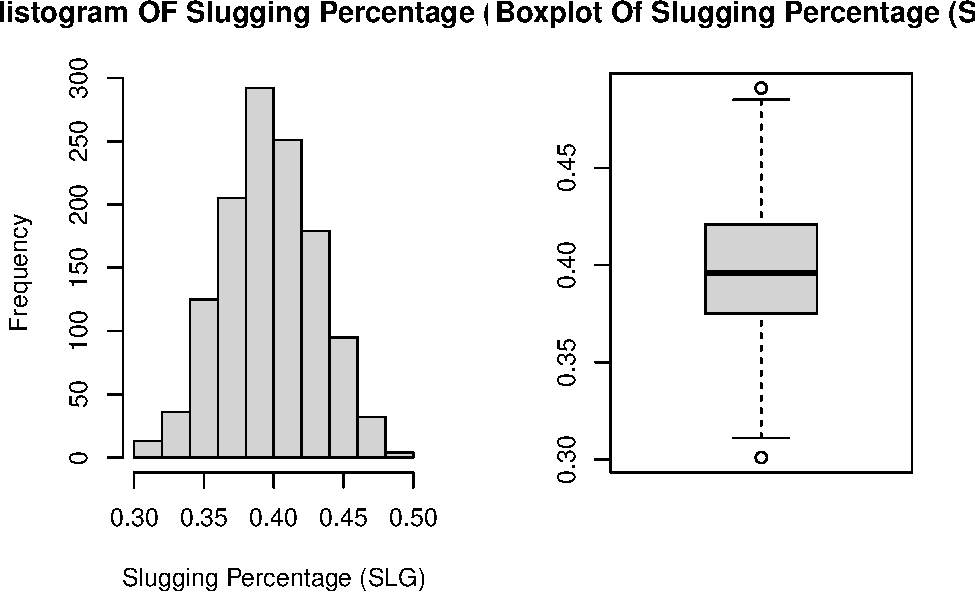
\includegraphics{HW2_Wu-Yulun_files/figure-latex/unnamed-chunk-12-2.pdf}

\begin{Shaded}
\begin{Highlighting}[]
\NormalTok{mean\_SLG }\OtherTok{=} \FunctionTok{mean}\NormalTok{(baseball}\SpecialCharTok{$}\NormalTok{SLG) }\CommentTok{\# Mean of SLG}
\FunctionTok{cat}\NormalTok{(}\StringTok{"The mean of SLG:"}\NormalTok{,mean\_SLG,}\StringTok{"}\SpecialCharTok{\textbackslash{}n}\StringTok{"}\NormalTok{)}
\end{Highlighting}
\end{Shaded}

\begin{verbatim}
## The mean of SLG: 0.3973417
\end{verbatim}

\begin{Shaded}
\begin{Highlighting}[]
\NormalTok{median\_SLG }\OtherTok{=} \FunctionTok{median}\NormalTok{(baseball}\SpecialCharTok{$}\NormalTok{SLG) }\CommentTok{\# Median of SLG}
\FunctionTok{cat}\NormalTok{(}\StringTok{"The median of SLG:"}\NormalTok{,median\_SLG,}\StringTok{"}\SpecialCharTok{\textbackslash{}n}\StringTok{"}\NormalTok{)}
\end{Highlighting}
\end{Shaded}

\begin{verbatim}
## The median of SLG: 0.396
\end{verbatim}

\begin{Shaded}
\begin{Highlighting}[]
\CommentTok{\# Histogram and Boxplot of BA}
\FunctionTok{par}\NormalTok{(}\AttributeTok{mfrow=}\FunctionTok{c}\NormalTok{(}\DecValTok{1}\NormalTok{,}\DecValTok{2}\NormalTok{))}
\FunctionTok{hist}\NormalTok{(baseball}\SpecialCharTok{$}\NormalTok{BA,}\AttributeTok{main=}\StringTok{"Histogram Of Batting Average (BA)"}\NormalTok{,}\AttributeTok{xlab=}\StringTok{"Batting Average (BA)"}\NormalTok{)}
\FunctionTok{boxplot}\NormalTok{(baseball}\SpecialCharTok{$}\NormalTok{BA,}\AttributeTok{main=}\StringTok{"Boxplot Of Batting Average (BA)"}\NormalTok{)}
\end{Highlighting}
\end{Shaded}

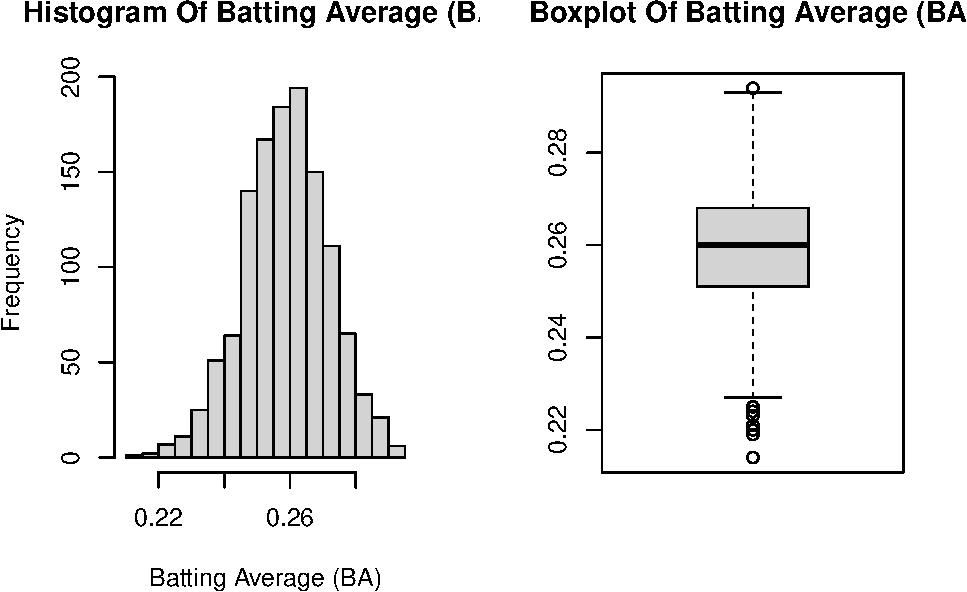
\includegraphics{HW2_Wu-Yulun_files/figure-latex/unnamed-chunk-12-3.pdf}

\begin{Shaded}
\begin{Highlighting}[]
\NormalTok{mean\_BA }\OtherTok{=} \FunctionTok{mean}\NormalTok{(baseball}\SpecialCharTok{$}\NormalTok{BA) }\CommentTok{\# Mean of BA}
\FunctionTok{cat}\NormalTok{(}\StringTok{"The mean of BA:"}\NormalTok{,mean\_BA,}\StringTok{"}\SpecialCharTok{\textbackslash{}n}\StringTok{"}\NormalTok{)}
\end{Highlighting}
\end{Shaded}

\begin{verbatim}
## The mean of BA: 0.2592727
\end{verbatim}

\begin{Shaded}
\begin{Highlighting}[]
\NormalTok{median\_BA }\OtherTok{=} \FunctionTok{median}\NormalTok{(baseball}\SpecialCharTok{$}\NormalTok{BA) }\CommentTok{\# Median of BA}
\FunctionTok{cat}\NormalTok{(}\StringTok{"The median of BA:"}\NormalTok{,median\_BA,}\StringTok{"}\SpecialCharTok{\textbackslash{}n}\StringTok{"}\NormalTok{)}
\end{Highlighting}
\end{Shaded}

\begin{verbatim}
## The median of BA: 0.26
\end{verbatim}

The mean of OBP is 0.3263312 and the median of OBP is 0.326, meaning
that the distribution of OBP is not skewed at all. The mean of SLG is
0.3973417 and the median of SLG is 0.396, meaning that the distribution
of SLG a little bit skew.

Part II

\begin{Shaded}
\begin{Highlighting}[]
\NormalTok{model1 }\OtherTok{=} \FunctionTok{lm}\NormalTok{(RS}\SpecialCharTok{\textasciitilde{}}\NormalTok{BA,}\AttributeTok{data=}\NormalTok{baseball) }\CommentTok{\# Marginal model RS\textasciitilde{}BA}
\FunctionTok{par}\NormalTok{(}\AttributeTok{mfrow=}\FunctionTok{c}\NormalTok{(}\DecValTok{1}\NormalTok{,}\DecValTok{2}\NormalTok{))}
\FunctionTok{plot}\NormalTok{(baseball}\SpecialCharTok{$}\NormalTok{BA, baseball}\SpecialCharTok{$}\NormalTok{RS,}\AttributeTok{main=}\StringTok{"RS v.s. BA"}\NormalTok{,}\AttributeTok{xlab=}\StringTok{"Batting Average (BA)"}\NormalTok{,}\AttributeTok{ylab=}\StringTok{"Runs Scored (RS)"}\NormalTok{) }\CommentTok{\# Scatter plot of RS v.s. BA}
\FunctionTok{abline}\NormalTok{(}\FunctionTok{summary}\NormalTok{(model1)}\SpecialCharTok{$}\NormalTok{coef[}\DecValTok{1}\NormalTok{],}\FunctionTok{summary}\NormalTok{(model1)}\SpecialCharTok{$}\NormalTok{coef[}\DecValTok{2}\NormalTok{],}\AttributeTok{col=}\StringTok{"blue3"}\NormalTok{) }\CommentTok{\# Fitted line}
\FunctionTok{qqnorm}\NormalTok{(}\FunctionTok{summary}\NormalTok{(model1)}\SpecialCharTok{$}\NormalTok{residuals, }\AttributeTok{pch =} \DecValTok{1}\NormalTok{, }\AttributeTok{frame =} \ConstantTok{FALSE}\NormalTok{,}\AttributeTok{main=}\StringTok{"Normal Q{-}Q plot of fitted residual of marginal model RS\textasciitilde{}BA"}\NormalTok{)}
\FunctionTok{qqline}\NormalTok{(}\FunctionTok{summary}\NormalTok{(model1)}\SpecialCharTok{$}\NormalTok{residuals, }\AttributeTok{col =} \StringTok{"steelblue"}\NormalTok{, }\AttributeTok{lwd =} \DecValTok{2}\NormalTok{)}
\end{Highlighting}
\end{Shaded}

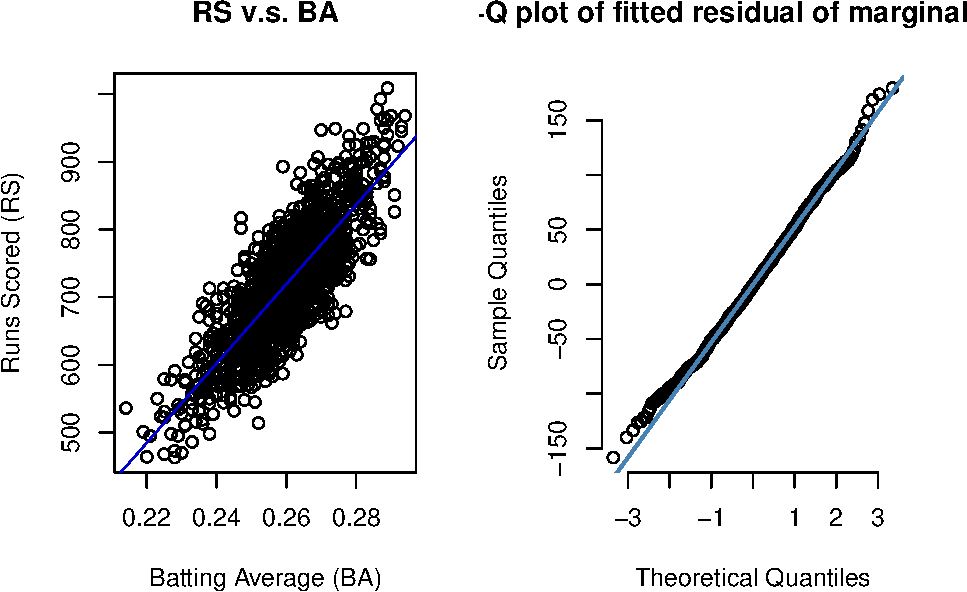
\includegraphics{HW2_Wu-Yulun_files/figure-latex/unnamed-chunk-13-1.pdf}

\begin{Shaded}
\begin{Highlighting}[]
\FunctionTok{cat}\NormalTok{(}\StringTok{"Fitted coefficient of model RS\textasciitilde{}BA is"}\NormalTok{,}\FunctionTok{summary}\NormalTok{(model1)}\SpecialCharTok{$}\NormalTok{coef[}\DecValTok{1}\NormalTok{],}\StringTok{","}\NormalTok{, }\FunctionTok{summary}\NormalTok{(model1)}\SpecialCharTok{$}\NormalTok{coef[}\DecValTok{2}\NormalTok{],}\StringTok{"}\SpecialCharTok{\textbackslash{}n}\StringTok{"}\NormalTok{)}
\end{Highlighting}
\end{Shaded}

\begin{verbatim}
## Fitted coefficient of model RS~BA is -805.511 , 5864.84
\end{verbatim}

\begin{Shaded}
\begin{Highlighting}[]
\FunctionTok{cat}\NormalTok{(}\StringTok{"R\^{}2 of marginal model of RS\textasciitilde{}BA is"}\NormalTok{,}\FunctionTok{summary}\NormalTok{(model1)}\SpecialCharTok{$}\NormalTok{r.squared,}\StringTok{"}\SpecialCharTok{\textbackslash{}n}\StringTok{"}\NormalTok{)}
\end{Highlighting}
\end{Shaded}

\begin{verbatim}
## R^2 of marginal model of RS~BA is 0.6839284
\end{verbatim}

\begin{Shaded}
\begin{Highlighting}[]
\NormalTok{model2 }\OtherTok{=} \FunctionTok{lm}\NormalTok{(RS}\SpecialCharTok{\textasciitilde{}}\NormalTok{OBP,}\AttributeTok{data=}\NormalTok{baseball) }\CommentTok{\# Marginal model RS\textasciitilde{}OBP}
\FunctionTok{par}\NormalTok{(}\AttributeTok{mfrow=}\FunctionTok{c}\NormalTok{(}\DecValTok{1}\NormalTok{,}\DecValTok{2}\NormalTok{))}
\FunctionTok{plot}\NormalTok{(baseball}\SpecialCharTok{$}\NormalTok{OBP, baseball}\SpecialCharTok{$}\NormalTok{RS,}\AttributeTok{main=}\StringTok{"RS v.s. OBP"}\NormalTok{,}\AttributeTok{xlab=}\StringTok{"On{-}Base Percentage (OBP)"}\NormalTok{,}\AttributeTok{ylab=}\StringTok{"Runs Scored (RS)"}\NormalTok{) }\CommentTok{\# Scatter plot of RS v.s. OBP}
\FunctionTok{abline}\NormalTok{(}\FunctionTok{summary}\NormalTok{(model2)}\SpecialCharTok{$}\NormalTok{coef[}\DecValTok{1}\NormalTok{],}\FunctionTok{summary}\NormalTok{(model2)}\SpecialCharTok{$}\NormalTok{coef[}\DecValTok{2}\NormalTok{],}\AttributeTok{col=}\StringTok{"blue3"}\NormalTok{) }\CommentTok{\# Fitted line}
\FunctionTok{qqnorm}\NormalTok{(}\FunctionTok{summary}\NormalTok{(model2)}\SpecialCharTok{$}\NormalTok{residuals, }\AttributeTok{pch =} \DecValTok{1}\NormalTok{, }\AttributeTok{frame =} \ConstantTok{FALSE}\NormalTok{,}\AttributeTok{main=}\StringTok{"Normal Q{-}Q plot of fitted residual of marginal model RS\textasciitilde{}OBP"}\NormalTok{)}
\FunctionTok{qqline}\NormalTok{(}\FunctionTok{summary}\NormalTok{(model2)}\SpecialCharTok{$}\NormalTok{residuals, }\AttributeTok{col =} \StringTok{"steelblue"}\NormalTok{, }\AttributeTok{lwd =} \DecValTok{2}\NormalTok{)}
\end{Highlighting}
\end{Shaded}

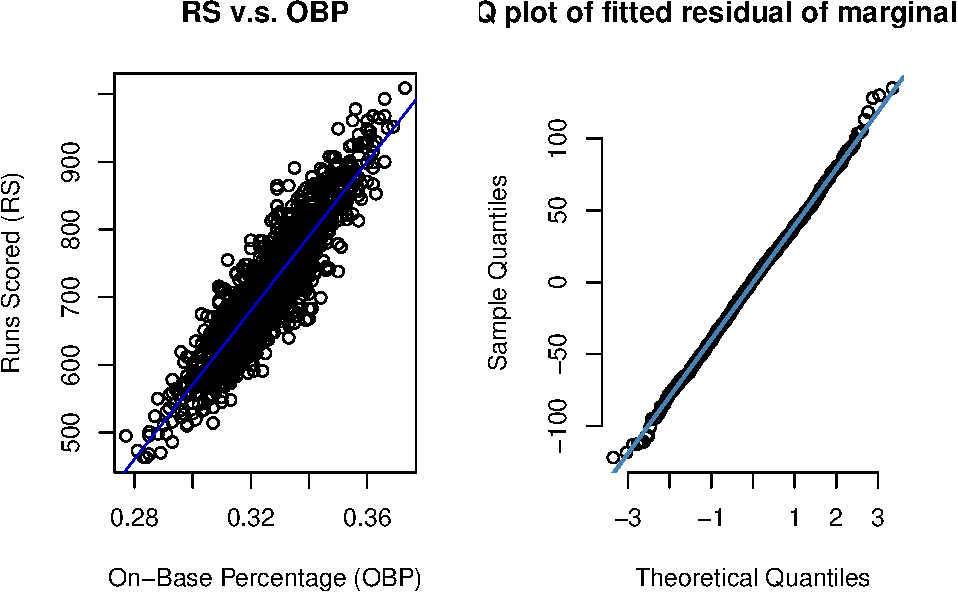
\includegraphics{HW2_Wu-Yulun_files/figure-latex/unnamed-chunk-13-2.pdf}

\begin{Shaded}
\begin{Highlighting}[]
\FunctionTok{cat}\NormalTok{(}\StringTok{"Fitted coefficient of model RS\textasciitilde{}OBP is"}\NormalTok{,}\FunctionTok{summary}\NormalTok{(model2)}\SpecialCharTok{$}\NormalTok{coef[}\DecValTok{1}\NormalTok{],}\StringTok{","}\NormalTok{, }\FunctionTok{summary}\NormalTok{(model2)}\SpecialCharTok{$}\NormalTok{coef[}\DecValTok{2}\NormalTok{],}\StringTok{"}\SpecialCharTok{\textbackslash{}n}\StringTok{"}\NormalTok{)}
\end{Highlighting}
\end{Shaded}

\begin{verbatim}
## Fitted coefficient of model RS~OBP is -1076.602 , 5490.386
\end{verbatim}

\begin{Shaded}
\begin{Highlighting}[]
\FunctionTok{cat}\NormalTok{(}\StringTok{"R\^{}2 of marginal model of RS\textasciitilde{}OBP is"}\NormalTok{,}\FunctionTok{summary}\NormalTok{(model2)}\SpecialCharTok{$}\NormalTok{r.squared,}\StringTok{"}\SpecialCharTok{\textbackslash{}n}\StringTok{"}\NormalTok{)}
\end{Highlighting}
\end{Shaded}

\begin{verbatim}
## R^2 of marginal model of RS~OBP is 0.8108862
\end{verbatim}

\begin{Shaded}
\begin{Highlighting}[]
\NormalTok{model3 }\OtherTok{=} \FunctionTok{lm}\NormalTok{(RS}\SpecialCharTok{\textasciitilde{}}\NormalTok{SLG,}\AttributeTok{data=}\NormalTok{baseball) }\CommentTok{\# Marginal model RS\textasciitilde{}SLG}
\FunctionTok{par}\NormalTok{(}\AttributeTok{mfrow=}\FunctionTok{c}\NormalTok{(}\DecValTok{1}\NormalTok{,}\DecValTok{2}\NormalTok{))}
\FunctionTok{plot}\NormalTok{(baseball}\SpecialCharTok{$}\NormalTok{SLG, baseball}\SpecialCharTok{$}\NormalTok{RS,}\AttributeTok{main=}\StringTok{"RS v.s. SLG"}\NormalTok{,}\AttributeTok{xlab=}\StringTok{"Slugging Percentage (SLG)"}\NormalTok{,}\AttributeTok{ylab=}\StringTok{"Runs Scored (RS)"}\NormalTok{) }\CommentTok{\# Scatter plot of RS v.s. SLG}
\FunctionTok{abline}\NormalTok{(}\FunctionTok{summary}\NormalTok{(model3)}\SpecialCharTok{$}\NormalTok{coef[}\DecValTok{1}\NormalTok{],}\FunctionTok{summary}\NormalTok{(model3)}\SpecialCharTok{$}\NormalTok{coef[}\DecValTok{2}\NormalTok{],}\AttributeTok{col=}\StringTok{"blue3"}\NormalTok{) }\CommentTok{\# Fitted line}
\FunctionTok{qqnorm}\NormalTok{(}\FunctionTok{summary}\NormalTok{(model3)}\SpecialCharTok{$}\NormalTok{residuals, }\AttributeTok{pch =} \DecValTok{1}\NormalTok{, }\AttributeTok{frame =} \ConstantTok{FALSE}\NormalTok{,}\AttributeTok{main=}\StringTok{"Normal Q{-}Q plot of fitted residual of marginal model RS\textasciitilde{}SLG"}\NormalTok{)}
\FunctionTok{qqline}\NormalTok{(}\FunctionTok{summary}\NormalTok{(model3)}\SpecialCharTok{$}\NormalTok{residuals, }\AttributeTok{col =} \StringTok{"steelblue"}\NormalTok{, }\AttributeTok{lwd =} \DecValTok{2}\NormalTok{)}
\end{Highlighting}
\end{Shaded}

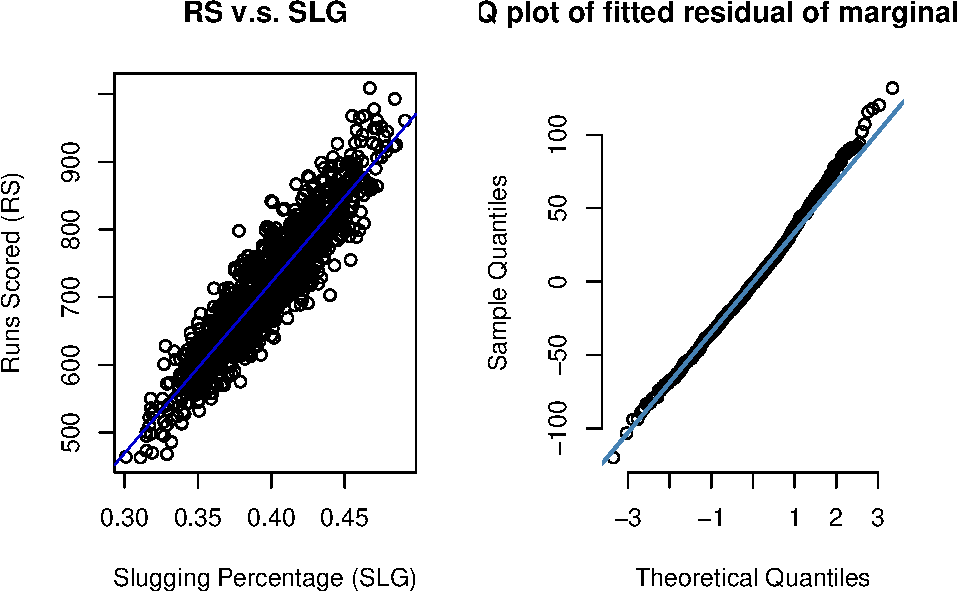
\includegraphics{HW2_Wu-Yulun_files/figure-latex/unnamed-chunk-13-3.pdf}

\begin{Shaded}
\begin{Highlighting}[]
\FunctionTok{cat}\NormalTok{(}\StringTok{"Fitted coefficient of model RS\textasciitilde{}SLG is"}\NormalTok{,}\FunctionTok{summary}\NormalTok{(model3)}\SpecialCharTok{$}\NormalTok{coef[}\DecValTok{1}\NormalTok{],}\StringTok{","}\NormalTok{, }\FunctionTok{summary}\NormalTok{(model3)}\SpecialCharTok{$}\NormalTok{coef[}\DecValTok{2}\NormalTok{],}\StringTok{"}\SpecialCharTok{\textbackslash{}n}\StringTok{"}\NormalTok{)}
\end{Highlighting}
\end{Shaded}

\begin{verbatim}
## Fitted coefficient of model RS~SLG is -289.368 , 2527.925
\end{verbatim}

\begin{Shaded}
\begin{Highlighting}[]
\FunctionTok{cat}\NormalTok{(}\StringTok{"R\^{}2 of marginal model of RS\textasciitilde{}SLG is"}\NormalTok{,}\FunctionTok{summary}\NormalTok{(model3)}\SpecialCharTok{$}\NormalTok{r.squared,}\StringTok{"}\SpecialCharTok{\textbackslash{}n}\StringTok{"}\NormalTok{)}
\end{Highlighting}
\end{Shaded}

\begin{verbatim}
## R^2 of marginal model of RS~SLG is 0.8440831
\end{verbatim}

\(R^2\) of marginal model of RS\textasciitilde BA is 0.6839284 which is
lower than \(R^2\) of RS\textasciitilde OBP and \(R^2\) of
RS\textasciitilde SLG, so this contradict to the intuition that BA is
thought to be most responsible for RS.

Part III

\begin{Shaded}
\begin{Highlighting}[]
\NormalTok{model4 }\OtherTok{=} \FunctionTok{lm}\NormalTok{(RS}\SpecialCharTok{\textasciitilde{}}\NormalTok{BA }\SpecialCharTok{+}\NormalTok{ SLG }\SpecialCharTok{+}\NormalTok{ OBP,}\AttributeTok{data=}\NormalTok{baseball)}
\FunctionTok{summary}\NormalTok{(model4)}\SpecialCharTok{$}\NormalTok{coef}
\end{Highlighting}
\end{Shaded}

\begin{verbatim}
##              Estimate Std. Error    t value      Pr(>|t|)
## (Intercept) -806.0845   17.39190 -46.348260 5.904672e-272
## BA          -134.9050  113.73431  -1.186141  2.357959e-01
## SLG         1533.8848   37.75868  40.623372 2.187242e-229
## OBP         2900.9403   97.87168  29.640243 4.386860e-146
\end{verbatim}

\begin{Shaded}
\begin{Highlighting}[]
\FunctionTok{cat}\NormalTok{(}\StringTok{"Since p{-}value of fitted coefficient of BA \textgreater{} 0.05, coefficient of BA is not significant.}\SpecialCharTok{\textbackslash{}n}\StringTok{"}\NormalTok{)}
\end{Highlighting}
\end{Shaded}

\begin{verbatim}
## Since p-value of fitted coefficient of BA > 0.05, coefficient of BA is not significant.
\end{verbatim}

\begin{Shaded}
\begin{Highlighting}[]
\FunctionTok{cat}\NormalTok{(}\StringTok{"All other fitted coefficients are significant.}\SpecialCharTok{\textbackslash{}n}\StringTok{"}\NormalTok{)}
\end{Highlighting}
\end{Shaded}

\begin{verbatim}
## All other fitted coefficients are significant.
\end{verbatim}

\begin{Shaded}
\begin{Highlighting}[]
\FunctionTok{cat}\NormalTok{(}\StringTok{"R\^{}2 of model of RS\textasciitilde{}BA + SLG + OBP is"}\NormalTok{,}\FunctionTok{summary}\NormalTok{(model4)}\SpecialCharTok{$}\NormalTok{r.squared,}\StringTok{"}\SpecialCharTok{\textbackslash{}n}\StringTok{"}\NormalTok{)}
\end{Highlighting}
\end{Shaded}

\begin{verbatim}
## R^2 of model of RS~BA + SLG + OBP is 0.9248834
\end{verbatim}

\begin{Shaded}
\begin{Highlighting}[]
\FunctionTok{qqnorm}\NormalTok{(}\FunctionTok{summary}\NormalTok{(model4)}\SpecialCharTok{$}\NormalTok{residuals, }\AttributeTok{pch =} \DecValTok{1}\NormalTok{, }\AttributeTok{frame =} \ConstantTok{FALSE}\NormalTok{,}\AttributeTok{main=}\StringTok{"Normal Q{-}Q plot of fitted residual of model RS\textasciitilde{}BA + SLG + OBP"}\NormalTok{)}
\FunctionTok{qqline}\NormalTok{(}\FunctionTok{summary}\NormalTok{(model4)}\SpecialCharTok{$}\NormalTok{residuals, }\AttributeTok{col =} \StringTok{"steelblue"}\NormalTok{, }\AttributeTok{lwd =} \DecValTok{2}\NormalTok{)}
\end{Highlighting}
\end{Shaded}

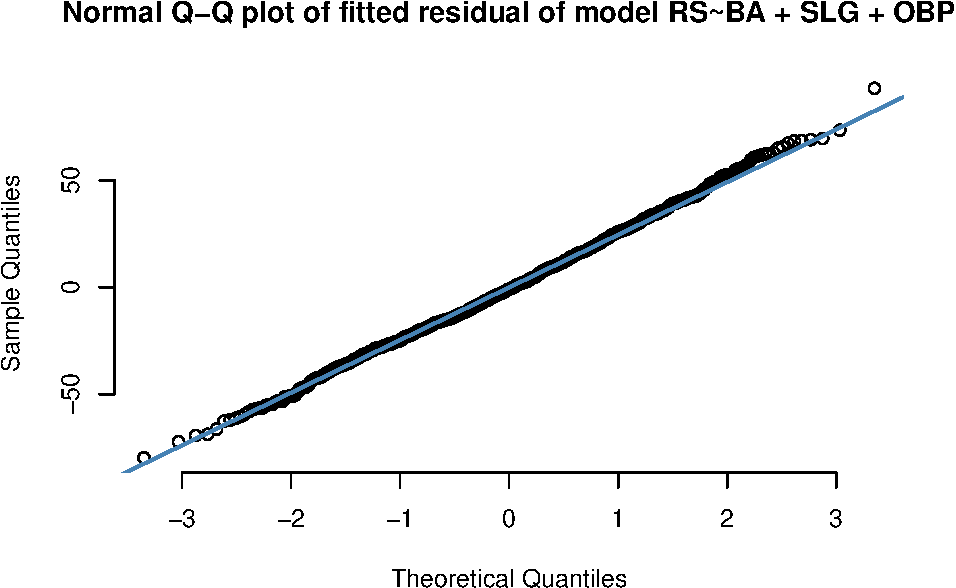
\includegraphics{HW2_Wu-Yulun_files/figure-latex/unnamed-chunk-14-1.pdf}

\begin{Shaded}
\begin{Highlighting}[]
\NormalTok{model5 }\OtherTok{=} \FunctionTok{lm}\NormalTok{(RS}\SpecialCharTok{\textasciitilde{}}\NormalTok{BA }\SpecialCharTok{+}\NormalTok{ SLG,}\AttributeTok{data=}\NormalTok{baseball)}
\FunctionTok{cat}\NormalTok{(}\StringTok{"R\^{}2 of model of RS\textasciitilde{}BA + SLG is"}\NormalTok{,}\FunctionTok{summary}\NormalTok{(model5)}\SpecialCharTok{$}\NormalTok{r.squared,}\StringTok{"}\SpecialCharTok{\textbackslash{}n}\StringTok{"}\NormalTok{)}
\end{Highlighting}
\end{Shaded}

\begin{verbatim}
## R^2 of model of RS~BA + SLG is 0.871143
\end{verbatim}

BA is not significant because its p-value = 2.357959e-01 \textless{}
0.05, this consist with the low \(R^2\) in marginal model
RS\textasciitilde BA in Part II. Also SLG and OBP are significant
consist with the high \(R^2\) in marginal model RS\textasciitilde SLG
and marginal model RS\textasciitilde OBP in Part II. Model
RS\textasciitilde BA + SLG + OBP is clearly better because it has a much
higher \(R^2\) than model of RS\textasciitilde BA + SLG.

Part IV

\begin{Shaded}
\begin{Highlighting}[]
\NormalTok{training\_baseball }\OtherTok{=}\NormalTok{ baseball[}\FunctionTok{which}\NormalTok{(baseball}\SpecialCharTok{$}\NormalTok{Year}\SpecialCharTok{\textless{}}\DecValTok{2002}\NormalTok{),]}
\NormalTok{training\_baseball[}\StringTok{"RD"}\NormalTok{] }\OtherTok{=}\NormalTok{ training\_baseball}\SpecialCharTok{$}\NormalTok{RS}\SpecialCharTok{{-}}\NormalTok{training\_baseball}\SpecialCharTok{$}\NormalTok{RA }\CommentTok{\# Add column RD=RS{-}RA }
\NormalTok{model6 }\OtherTok{=} \FunctionTok{lm}\NormalTok{(W }\SpecialCharTok{\textasciitilde{}}\NormalTok{ RD,}\AttributeTok{data=}\NormalTok{training\_baseball) }\CommentTok{\# Model of W \textasciitilde{} RD}
\NormalTok{model7 }\OtherTok{=} \FunctionTok{lm}\NormalTok{(RS}\SpecialCharTok{\textasciitilde{}}\NormalTok{OBP }\SpecialCharTok{+}\NormalTok{ SLG,}\AttributeTok{data=}\NormalTok{training\_baseball) }\CommentTok{\# Model of RS\textasciitilde{}OBP + SLG}
\NormalTok{model8 }\OtherTok{=} \FunctionTok{lm}\NormalTok{(RA}\SpecialCharTok{\textasciitilde{}}\NormalTok{OOBP }\SpecialCharTok{+}\NormalTok{ OSLG,}\AttributeTok{data=}\NormalTok{training\_baseball) }\CommentTok{\# Model of RA\textasciitilde{}OOBP + OSLG}

\CommentTok{\# Create dataframe for Xnew}
\NormalTok{OBP }\OtherTok{=} \FloatTok{0.349}
\NormalTok{SLG }\OtherTok{=} \FloatTok{0.430}
\NormalTok{OOBP }\OtherTok{=} \FloatTok{0.307}
\NormalTok{OSLG }\OtherTok{=} \FloatTok{0.373}
\NormalTok{Xnew }\OtherTok{=} \FunctionTok{data.frame}\NormalTok{(OBP,SLG,OOBP,OSLG)}
\NormalTok{Xnew}
\end{Highlighting}
\end{Shaded}

\begin{verbatim}
##     OBP  SLG  OOBP  OSLG
## 1 0.349 0.43 0.307 0.373
\end{verbatim}

\begin{Shaded}
\begin{Highlighting}[]
\NormalTok{RA\_pred }\OtherTok{=} \FunctionTok{predict}\NormalTok{(model8,Xnew) }\CommentTok{\# Predicted RA}
\NormalTok{RA\_pred}
\end{Highlighting}
\end{Shaded}

\begin{verbatim}
##        1 
## 621.9258
\end{verbatim}

\begin{Shaded}
\begin{Highlighting}[]
\NormalTok{RS\_pred }\OtherTok{=} \FunctionTok{predict}\NormalTok{(model7,Xnew) }\CommentTok{\# Predicted RS}
\NormalTok{RS\_pred}
\end{Highlighting}
\end{Shaded}

\begin{verbatim}
##        1 
## 832.3647
\end{verbatim}

\begin{Shaded}
\begin{Highlighting}[]
\NormalTok{RD }\OtherTok{=}\NormalTok{ RS\_pred}\SpecialCharTok{{-}}\NormalTok{RA\_pred }\CommentTok{\# Predicted RD}
\NormalTok{W\_pred }\OtherTok{=} \FunctionTok{predict}\NormalTok{(model6,}\FunctionTok{data.frame}\NormalTok{(RD)) }\CommentTok{\# Predicted W}
\FunctionTok{cat}\NormalTok{(}\StringTok{"Oakland Athletics is predicted to have"}\NormalTok{,W\_pred,}\StringTok{"win games in 2002."}\NormalTok{)}
\end{Highlighting}
\end{Shaded}

\begin{verbatim}
## Oakland Athletics is predicted to have 103.1386 win games in 2002.
\end{verbatim}

\begin{Shaded}
\begin{Highlighting}[]
\FunctionTok{cat}\NormalTok{(}\StringTok{"The true number of win games for Oakland Athletics in 2002 is"}\NormalTok{,baseball[}\FunctionTok{which}\NormalTok{(baseball}\SpecialCharTok{$}\NormalTok{Year}\SpecialCharTok{==}\DecValTok{2002}\SpecialCharTok{\&}\NormalTok{baseball}\SpecialCharTok{$}\NormalTok{Team}\SpecialCharTok{==}\StringTok{"OAK"}\NormalTok{),}\StringTok{"W"}\NormalTok{])}
\end{Highlighting}
\end{Shaded}

\begin{verbatim}
## The true number of win games for Oakland Athletics in 2002 is 103
\end{verbatim}

\begin{Shaded}
\begin{Highlighting}[]
\FunctionTok{cat}\NormalTok{(}\StringTok{", which is the same as our prediction after round our prediction to integer."}\NormalTok{,}\StringTok{"}\SpecialCharTok{\textbackslash{}n}\StringTok{"}\NormalTok{)}
\end{Highlighting}
\end{Shaded}

\begin{verbatim}
## , which is the same as our prediction after round our prediction to integer.
\end{verbatim}

\end{document}
